\documentclass[openany,a4paper,11pt]{book}
%Das ist die Zusammenfassung für die Vorlesung "Nichtlineare Regelungssysteme" im Sommersemester 2016. Es basiert auf das Skript vom Demirdelen und die Literaturen.

\usepackage{geometry}
\geometry{left=2.65cm,right=2.65cm,top=1.69cm,bottom=2.6cm,headsep=0.1cm,foot=1cm} 
\usepackage[T1]{fontenc}
\usepackage[utf8]{inputenc}
\usepackage{lmodern}
\usepackage{hyperref}
\usepackage{graphicx}
\usepackage{ulem}
\usepackage[english,ngerman]{babel} 
\usepackage{epic}
\usepackage{tikz}
\usetikzlibrary{shapes,arrows}
\usepackage{amsfonts}
\usepackage{amsmath}

\hyphenpenalty=5000
\tolerance=1000

\title{\Huge \textbf{Nichtlineare Regelungssysteme}\\[2cm] \protect 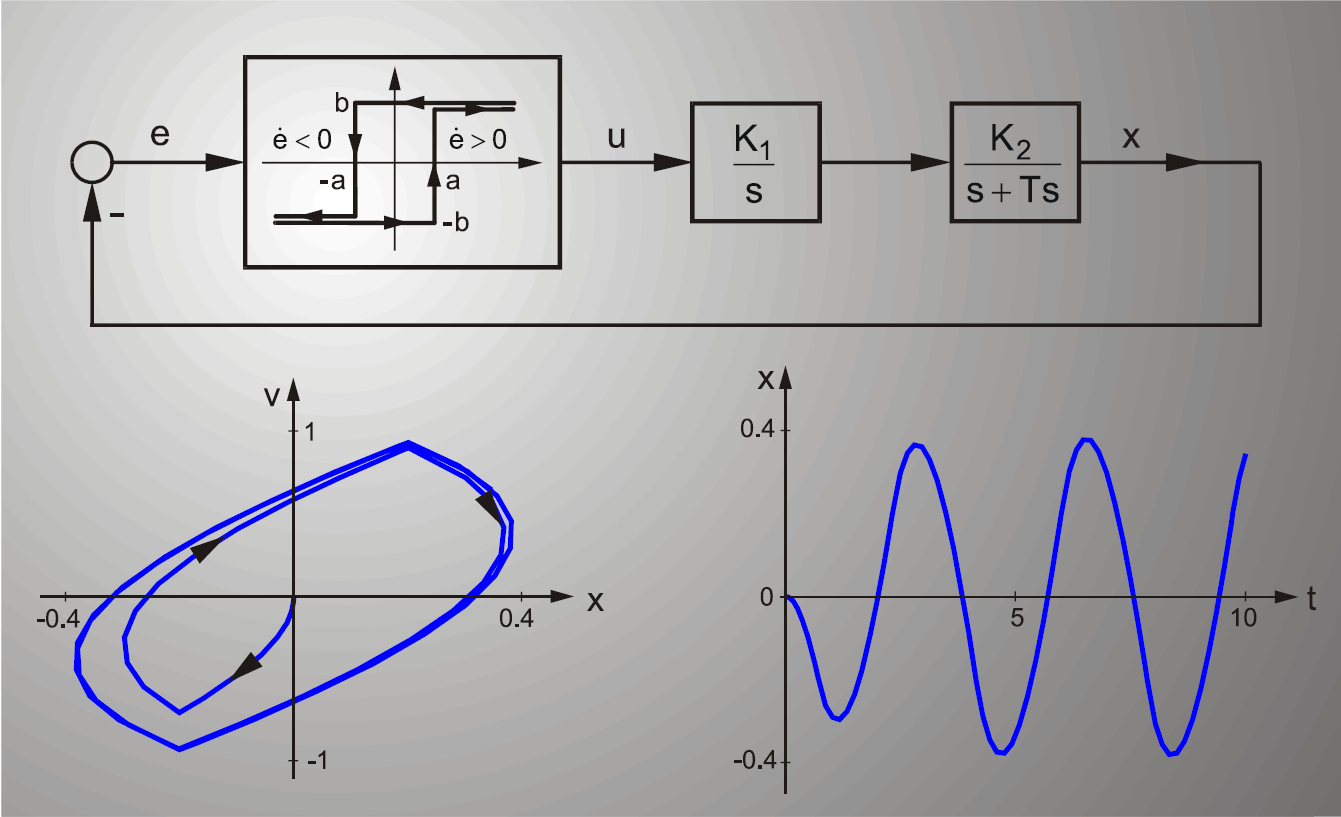
\includegraphics[width=\textwidth]{imgs/nlr.png}}
\author{Jun Lou}
\date{4. September 2016}

\begin{document}
%\linespread{1.1} 
%\pagestyle{plain}
\maketitle 
\pagestyle{plain}
%---------------------------Vorwort-----------------------------%
\addcontentsline{toc}{chapter}{Vorwort}
\chapter*{Vorwort}   
Dieses Skript geh"ort zur Vorlesung „Nichtlineare Regelungssysteme“ vom Herrn Dr. Mathias Kluwe am Karlsruher Institut für Technologie (KIT), die ich im Sommersemester 2016 gehalten habe. Inhaltlich habe ich mich dabei an die Abschrift aus der Fachschaft gehalten. \\[5pt]
Leider ist es nicht ausgeschlossen (nat"urlich), dass sich trotz sorgf"altiger Durchsicht noch Fehler verbergen. Wer Lust hat ein wenig Korrektur zu lesen, oder wer Fehler, besonders inhaltlicher Art im Skript entdeckt, teile es mir bitte mit: {\color{blue}\href{mailto:jun.lou.chn@outlook.com}{jun.lou.chn@outlook.com}}\\[5pt]
Das Skript ist nur für den persönlichen Gebrauch der Studierenden der Mechatrinik/ Elektrotechnik und Informationstechnik am KIT vorgesehen und darf nicht in irgendeiner Art und Weise vervielfältigt oder ver"offentlicht werden. \\[5pt]
Fur Kritik und Anregungen bin ich jederzeit dankbar.\\[6pt]
\begin{flushright} Jun Lou, am 4. September 2016\\
in Karlsruhe\end{flushright}

\tableofcontents
%\makeatletter
%--------------------------Kapitel 1----------------------------%
\chapter[Grundlagen]{Grundlagen}
\section[Grundlagen]{Nichtlineare Systeme-Definition, Beschreibung und typische Strukturen}
\uline{Definition: Nichtlineare Systeme (NLS):} \fbox{s. BB imgs/NLR 1-1, 1-2} \\
\uline{Beispiel: Gleichstromotor:} \fbox{s. BB imgs/NLR 1-3, 1-4} \\
\uline{typische Nichtlinearitäten:}
\begin{itemize}
    \item Kennlinienglieder: $y=F(u)$  
    \item{Multilizierhglieder:$y=K \cdot u_1 \cdot u_2$}
\end{itemize}
allgemein: \fbox{$y=F(u_1,u_2,...)$}\\
\uline{häufig für technische Anwendungen:} Einbettung von statischen Nichtlinearitäten in ein lineares Grundgrüst, welches die Dynamik bestimmt.\\
\uline{Beispiel 1: Nichtlinearer Regelkreis}\\
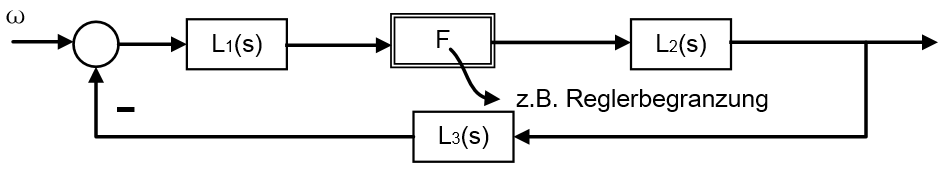
\includegraphics[height=0.9in]{imgs/NLR1.png}\\
\uline{Beispiel 2: Temperaturregelung}\\
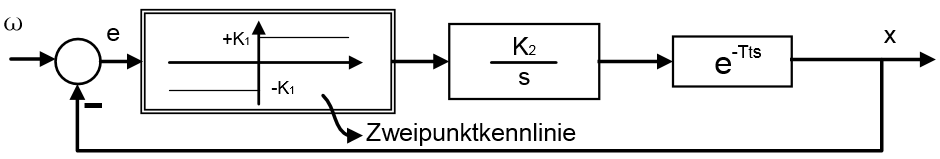
\includegraphics[height=0.8in]{imgs/NLR2.png}\\
\uline{Zweipunktkennlinie}\\
 $u = \left \{%
\begin{array}{lcrcl}
     K_1 & ,e>0 \\
     -K_1 & ,e<0 \\
\end{array} \right.$ \\
Amplitude:  $A=K_1\cdot K_2\cdot T_t $ ; Periodendauer: $T_p=4 \cdot T_t$ \\
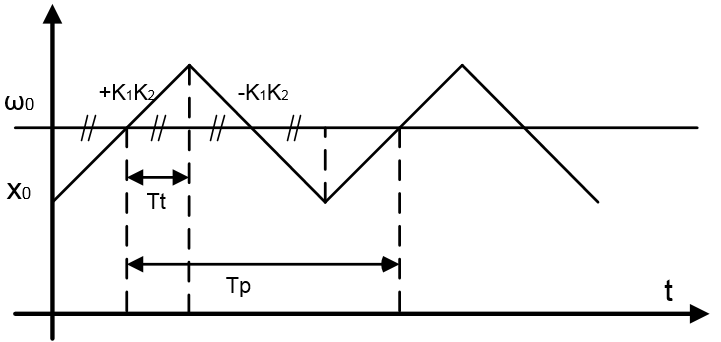
\includegraphics[height=1.6in]{imgs/NLR3.png}\\
\uline{also:} 
\begin{itemize}
    \item Schwingung unabhängig von äußeren Einflussen ($x_0$), bestimmt durch Systemparameter.
    \item Bei nicht zu großen Systemparameteränderungen bleibt Dauerschwingung erhalten. 
\end{itemize}
Hier verwendete \uline{Beschreibungsform von dynamischen Systeme}.\\
\uline{Zustandsraumdarstellung} (im allgemeinen Form) \fbox{s. BB imgs/NLR 1-5 bis 1-8}
\section[Grundlagen]{Stabilitätsbegriff bei nichtlinearen Systemen}
\begin{tabular}{ll}
\uline{bekannt:} & - Übertragungsstabilität\\
& - Stabilität bezüglich Anfangsauslenkungen(aus Ruhelagen)\\
\end{tabular}
\begin{enumerate}
    \item \uline{Übertragungsstabilität}\\
    Lineare Systeme ($g(t)$, $G(s)$)\\
    System $y(t)=\varphi u(t)=g(t)*u(t)$ stabil, wenn gilt:
   \[\int_{0}^{\infty} |g(\tau)|d\tau < +\infty \Leftrightarrow \forall t: |u(t)|\le M_1 \\ \Rightarrow |y(t)|\le M_2 \]
    \uline{Nichtlineare Systeme:}\\
    ungleich schwinger, die keine Faltung definiert\\
    Komplexe Begriffe aus der Funktionalanalysis erfordlich (z.B. Norm $||u||_2=[\int_{0}^{\infty}u^2(t)dt]^{\frac{1}{2}}$ dem System stabil, wenn $||y||_2\le \varphi||u||_2$)\\
    \uline{aber:} wegen zu hohen mathematischen Aufwendes nicht verwendet\\
    \uline{hier: Stabilität von Ruhelagen betrachtet}
    \item \uline{Stabilität von Ruhelagen}\\
    \uline{Definition: Ruhelage} \fbox{s. BB imgs/NLR 1-9} \\
    \begin{tabular}{ll}
    \uline{häufig:} & Ruhelage = Betriebszustand, Arbeitspunkt\\
    & $\Rightarrow$ Betrachtung des Systems in der Umgebung der Ruhelage gerechtfertigt!\\
    \end{tabular}
    \uline{Spezialfall:} \uline{Nichtlinearer Regelkreis} \fbox{s. BB imgs/NLR 1-10 bis 1-14} \\
    \uline{Lineare Systeme:} Ruhelage $\uline{x}_R$ aus $\uline{0}=\uline{A}\cdot\uline{x}_R+\uline{B}\cdot\uline{u}_R$\\
    $\Rightarrow$ 3 Arten von Ruhelagen möglich: \\
    \begin{tabular}{ll}
    - det $\uline{A} \ne 0$:& 1)genau eine Ruhelage: $\uline{x}_R=-\uline{A}^{-1}\cdot\uline{B}\cdot\uline{u}_R$\\
    - det $\uline{A} = 0$:& 2) keine Ruhelage (nicht möglich für $\uline{u}_R=\uline{0}$)\\
    & 3) unendlich viele Ruhelagen (Unterraum des Zustandsraums)\\
    \end{tabular}
\end{enumerate}
\uline{Nichtlineare Systeme:} auch mehrere, aber endlich viele Ruhelagen möglich\\
\uline{Beispiel: Pendel}
\[m\cdot\ddot{s}=-mg\cdot sin\varphi (s=R\cdot \varphi) \Rightarrow \ddot {\varphi}= -\frac{g}{R}\cdot sin\varphi\]
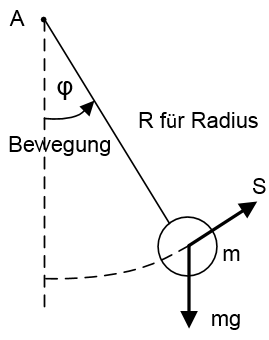
\includegraphics[width=1.4in]{imgs/NLR4.png}\\
Wahl: $x_1=\varphi, x_2=\dot{\varphi} \Rightarrow$
\[\left.
\begin{array}{r}
\dot{x}_1 = x_2\\
\dot{x}_2=-\frac{g}{R}\cdot sin{x_1}
\end{array}
\right\} \Rightarrow \text{\uline{2 Ruhelagen:}}\, (0,0), (\pi,0) \]
\uline{Stabilität nach Lyapunov} \fbox{s. BB imgs/NLR 1-15} \\
Ruhelage ($\mathbb{R}_2$)
\begin{table}[htbp]
    \centering
    \begin{tabular}{ccc}
     \uline{stabil} &\uline{instabil} & \uline{asymptotisch stabil}  \\
     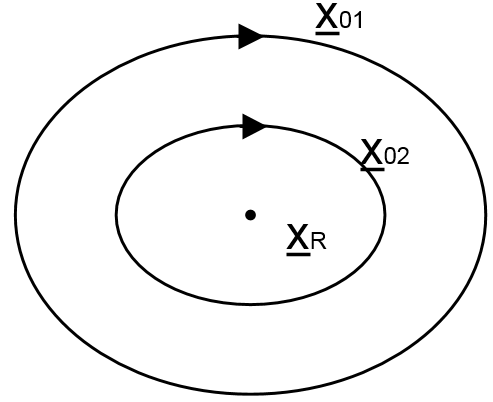
\includegraphics[width=1.5in]{imgs/NLR5.png} & 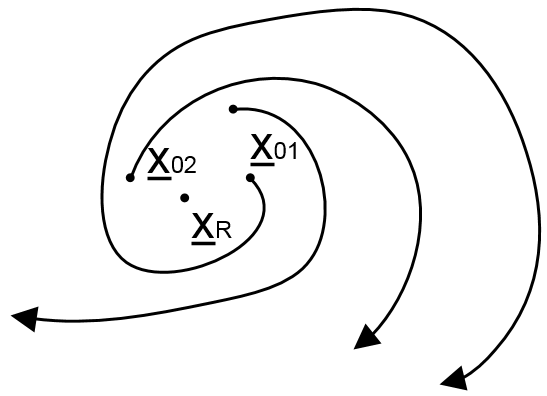
\includegraphics[width=1.5in]{imgs/NLR6.png} & 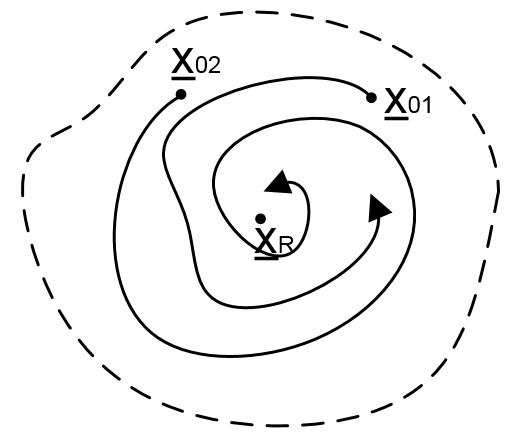
\includegraphics[width=1.5in]{imgs/NLR7.png} \\
    \end{tabular}
\end{table}
\uline{Beispiel: Pendel} \fbox{s. BB imgs/NLR 1-16} \\
charakteristisch für nichtlineare Systeme
\begin{itemize}
    \item Ruhelagen mit unterschiedlichen Stabilitätsverhalten möglich.
    \item Ruhelage kann \uline{asymptotisch stabil} sein, \uline{ohne global asymptotisch stabil} zu sein.
\end{itemize}
%--------------------------Kapitel 2----------------------------%
\chapter[Analyse \& Synthese in der Zustandsebene]{Analyse und Synthese nichtlinearer System in der Zustandsebene}
\uline{Prinzip:} Bestimmung der Trajaktorienverläufe, \uline{aber} ab $\mathbb{R}^3$ schwierig\\
$\Rightarrow$ Beschreibung auf Differentialgleichungen 2. Ordnung (Trajektorien beschreiben Kurven in der (x,v)-Ebene)
\section{Prinzipielle Vorgehensweise}
\[\begin{split}
\ddot{x}=f(x,&\dot{x},u)\\
\Downarrow &\text{Wahl der Zustandsvariablen:}  \quad x, v=\dot{x}\\
\left.
\begin{array}{r}
\dot{x}=v\\
\dot{v}=\ddot{x}=f(x,v,u)
\end{array}
\right\} &\text{Zustandsdifferentialgleichung}   
\end{split} \]
$\Rightarrow$ Zustandsebene = \uline{Phasenebene}\\
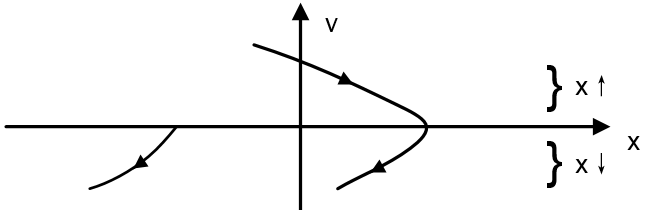
\includegraphics[width=3.5in]{imgs/NLR8.png} \\
$\Rightarrow$ Zustandsdifferentialgleichungen bilden autonomes System\\
\uline{Annahme:} u stückweise konstant \\
$\Rightarrow$ Reduktion auf eine Differentialgleichung 1. Ordnung möglich
\[\frac{\dot{v}}{\dot{x}}=\frac{\frac{dv}{dt}}{\frac{dx}{dt}}=\frac{dv}{dx}=\frac{f(x,v,u)}{v} \Rightarrow \text{Eine Differenzialgleichung für } v=v(x) \text{ oder } x=x(v)\]
\uline{Beispiel: Pendel} \fbox{s. BB imgs/NLR 2-1, 2-2}\\
in $\frac{dv}{dx}=\frac{f(x,v,u)}{v}$  Verlust der direkten Zeitabhängigkeit, berechenbar aus \uline{Zeitformeln:}
\[t_{0e} \text{ aus: }\text{a)}\quad \dot{x}=\frac{dx}{dt}=v(x) \Rightarrow \int_{t_0}^{t_e}dt=\int_{x_0}^{x_e}\frac{dx}{v(x)}=t_{0e}\]
\[\text{b)}\quad \dot{v}=\frac{dv}{dt}=f(x,v,u) \Rightarrow \int_{t_0}^{t_e}dt=\int_{v_0}^{v_e}\frac{dv}{f(x,v,u)}=t_{0e}\]
\uline{Spezialfälle:}
\begin{itemize}
    \item Lineares System: $\ddot{x}=f(x,\dot{x},u) \Rightarrow \ddot{x}+a_1\dot{x}+a_0x= u$
    \item Steuergröße $u$ stückweise konstant $\Rightarrow \uline{\ddot{x}+a_1\dot{x}+a_0x=c} \quad \quad (*)$
\end{itemize}
\uline{Beispiel für (*):} $a_1=a_0=0: \quad \uline{\ddot{x}=c}\quad \Rightarrow \left.
\begin{array}{r}
\dot{x}=v\\
\dot{v}=c
\end{array}
\right\} \frac{dv}{dx}=\frac{c}{v}$\\
Trennung der Veränderlichen: $\int vdv=\int cdx $\\
$\Rightarrow$ \fbox{$v^2=2cx+konst$}  \quad \uline{Parabeln} in der Phasenebene\\
\uline{dabei:} Scheitelpunkt ($x_s$,0): $0=2cx_s+konst \Rightarrow v^2=2c(x-x_s)$\\
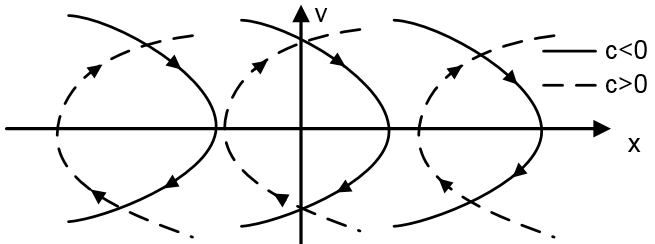
\includegraphics[height=1.2in]{imgs/NLR9.png}\\
\uline{Trajektorienverläufe weiterer linearen Systeme:} \fbox{s. BB imgs/NLR 2-3 bis 2-12}
\section[Trajektorien \& Stabilität der Ruhelagen]{Trajektorien des nichtlinearen Standardregelkreises in der Phasenebene und Stabilität der Ruhelagen}
\uline{Struktur:} \fbox{s. BB imgs/NLR 1-13}\\
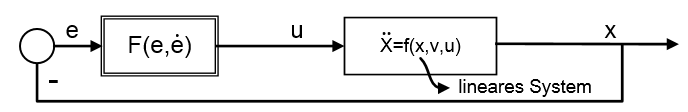
\includegraphics[width=4.4in]{imgs/NLR10.png}\\
\uline{hier:} Nichtlinear-Glied: $F(e,\dot{e})$: Kennlinien\\
(auch weitere typische Nichtliearitäten denkbar:\fbox{s. BB imgs/NLR 2-13 bis 2-15})\\
\uline{1. Beispiel:} ungedämpfte Lageregelstrecke\\
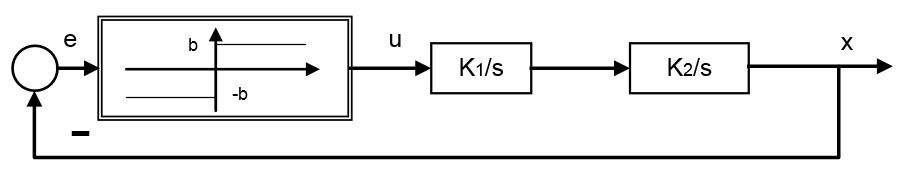
\includegraphics[width=4.4in]{imgs/NLR11.png}
\[\ddot{x}=K_1\cdot K_2\cdot u \quad 
\left.
\begin{array}{r}
\dot{x}=v\\
\dot{v}=K_1\cdot K_2\cdot u
\end{array}
\right\} \Rightarrow \frac{dv}{dx}=\frac{K_1\cdot K_2\cdot u}{v} \]
$\Rightarrow$ s. früher (Abschnitt 2.1) Trajektorien: Parabeln \fbox{$v^2=2K_1\cdot K_2\cdot u(x-x_s)$}\\
\uline{Stellgröße $u$:} konstant in Abhängigkeit von \uline{Schaltbedingungen}\\
$u = \left \{%
\begin{array}{lcrcl}
     -b & ,e<0 & \text{d.h.} \quad x>0 \\
     b & ,e>0 & \text{d.h.} \quad x<0 \\
\end{array} \right.$ \\
\uline{Schwingungsperiode $T_p$}\\
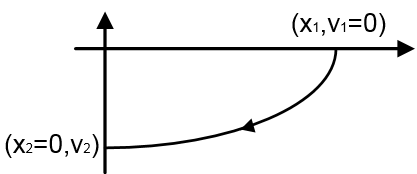
\includegraphics[width=1.6in]{imgs/NLR12.png} 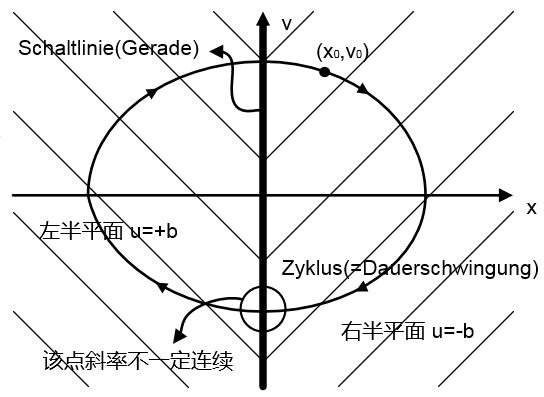
\includegraphics[width=3in]{imgs/NLR13.png}\\
Symmetrie: $T_p=4\cdot t_{12}$\\
\uline{allgemein:} \[v^2=2K_1\cdot K_2\cdot u(x-x_s) \stackrel{(u=-b, x_1=x_s)}{\Rightarrow} v^2=2K_1 \cdot K_2 \cdot b \cdot (x_1-x)\]
\[\Rightarrow v=-\sqrt{2K_1 \cdot K_2 \cdot b \cdot (x_1-x)}\]
\[\dot{v}=\frac{dv}{dt}=- K_1 \cdot K_2 \cdot b \quad \text{\uline{also:}} \quad \int_{t_1}^{t_2}dt=\int_{v_1}^{v_2}\frac{dv}{- K_1 \cdot K_2 \cdot b}\]
\[t_{12}=-\frac{v}{K_1 \cdot K_2 \cdot b} \bigg|_{v_1}^{v_2} \quad \text{mit} \quad 
\left \{%
\begin{array}{lcrcl}
     v_1=0\\
     v_2=-\sqrt{2K_1 \cdot K_2 \cdot b\cdot x_1}\\
\end{array} \right. \]
\[=\frac{\sqrt{2K_1 \cdot K_2 \cdot b\cdot x_1}}{K_1 \cdot K_2 \cdot b}=\sqrt{\frac{2x_1}{K_1 \cdot K_2 \cdot b}}\]
\[T_p=4\cdot t_{12}=4\sqrt{\frac{2x_1}{K_1 \cdot K_2 \cdot b}}\]
\uline{Stabilität der Ruhelage:} aus Regelkreis ablesbar: einzige Ruhelage $\uline{x}_R$=(0,0) bei $\uline{x}_0\ne\uline{0}$ bahnstabile Dauerschwingungen.\\
$\Rightarrow$ $\uline{x}_R$ stabil, aber nicht asymptotisch stabil\\
\uline{Verbesserung des Stabilitätsverhaltens}\\
\uline{Schrägstellung der Schaltlinie}\\
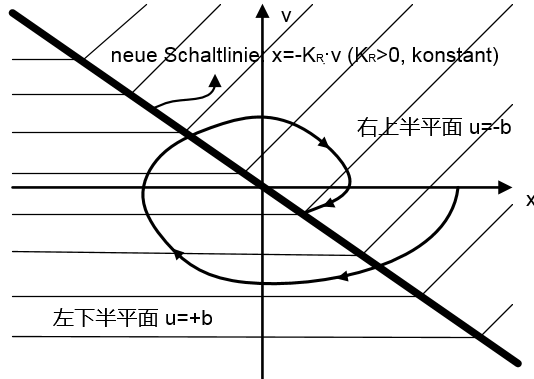
\includegraphics[width=3in]{imgs/NLR14.png}\\
\uline{neue Schaltbedingungen}
\[u = \left \{%
\begin{array}{lcrcl}
     -b & ,x>-K_R\cdot v & \text{bzw.}\quad x+K_R\cdot v>0 &\\
     b & ,x<-K_R\cdot v & \text{bzw.}\quad x+K_R\cdot v<0 &u=b\cdot sgn[-(x+K_R\cdot v)] \\
\end{array} \right.
\]
\uline{Realisierung dieses Schaltgesetzes:}
\begin{enumerate}
    \item \uline{zusätzliche Rückführung:}\\
    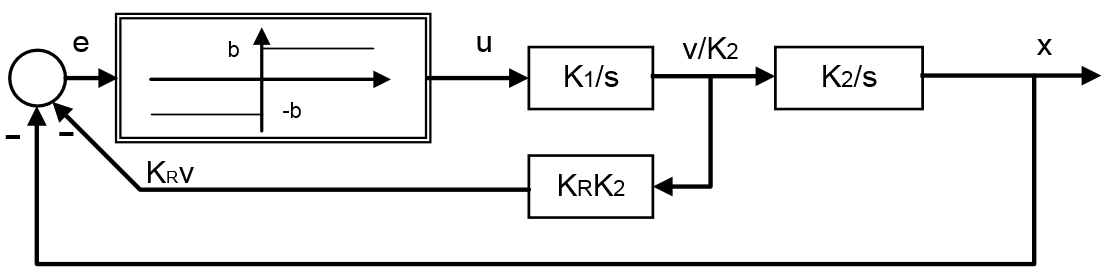
\includegraphics[width=4.2in]{imgs/NLR15.png}
    \item \uline{zusätzliche Parallelschaltung:}\\
    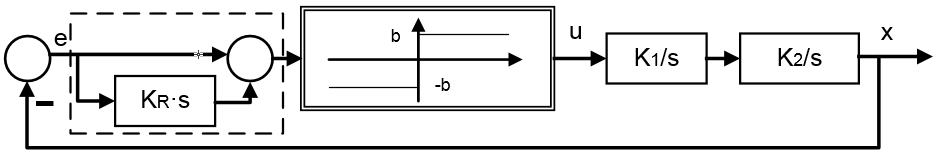
\includegraphics[width=4.4in]{imgs/NLR16.png}
\end{enumerate}
\uline{Problem:} Auftreten von Gleitvorgängen\\
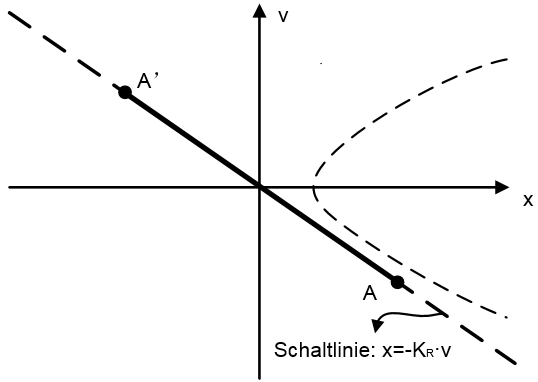
\includegraphics[width=2.5in]{imgs/NLR17.png}\\
Zustandspunkt kann die Schaltlinie zwischen A und O nicht mehr verlassen.\\
$\Rightarrow x=-K_R\cdot \dot{x}\quad \Rightarrow \quad K_R\cdot \dot{x}+x=0\quad \Rightarrow \quad x(t)=c\cdot e^{-\frac{t}{K_R}}$\\
Kriechvorgang nach \uline{0} und oszilliert $\rightarrow$ sehr problematisch\\
$\Rightarrow$ also: Schaltlinie nicht zu stark neigen, um die Strapazierung der Stellenrichtung zu vermeiden.\\
Situationen: \fbox{s. BB imgs/NLR 2-16, 2-17}\\
\uline{2. Beispiel:} gedämpfte Lageregelstrecke\\
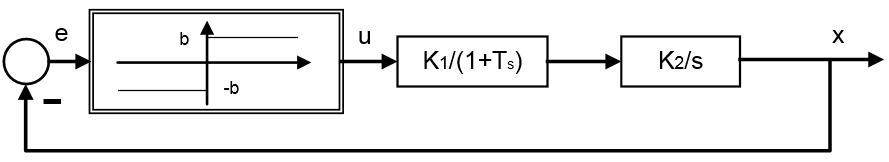
\includegraphics[width=4.6in]{imgs/NLR18.png}
\[X(s)=\frac{K_1 \cdot K_2}{Ts^2+s}U(s) \quad \Rightarrow \quad T\cdot\ddot{x}(t)+\dot{x}(t)=K_1\cdot K_2\cdot u(t)\]
\begin{tabular}{ll}
\uline{Zuständsgrößen:} & $\dot{x}=v$\\
& $\dot{v}=\frac{K_1 K_2 u-v}{T}$\\
\end{tabular}
\uline{Trajektorien:} Vergleich mit \fbox{BB imgs/NLR 2-4, 2-5}\\
hier Spezialfall 1$\beta$) Situationen: \fbox{s. BB imgs/NLR 2-18}
\[u = \left \{%
\begin{array}{lcrcl}
     -b & ,x=-T\cdot v+K_1\cdot K_2\cdot b\cdot T\cdot ln|v+K_1\cdot K_2\cdot b|+c_1\\
     +b & ,x=-T\cdot v-K_1\cdot K_2\cdot b\cdot T\cdot ln|v-K_1\cdot K_2\cdot b|+c_2\\
\end{array} \right.\]
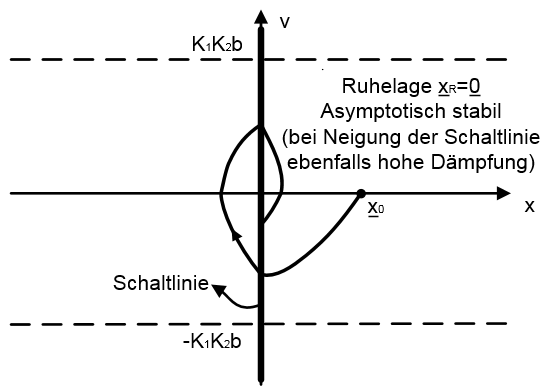
\includegraphics[width=2.6in]{imgs/NLR19.png}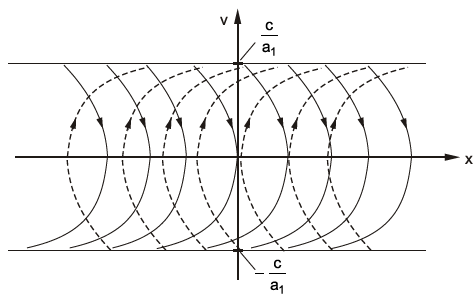
\includegraphics[width=2.8in]{imgs/NLR19_1.png}
\section{Strukturumschaltung}
\uline{bisher:} Nichtlineare Blöcke im Regelkreis vorhanden(s. Bsp. 2 von 2.2), die die Ruhelage asymptotisch stablisieren.\\
\uline{Idee:} Verbesserung des Stabilitätsverhaltens eines linearen Regelkreises durch \uline{Strukturumschaltung} (=Veränderung von Reglerparametern während des Betreibs)(= nichtlineares Verhalten)\\
\uline{Beispiel:} Umschaltender P-Regler\\
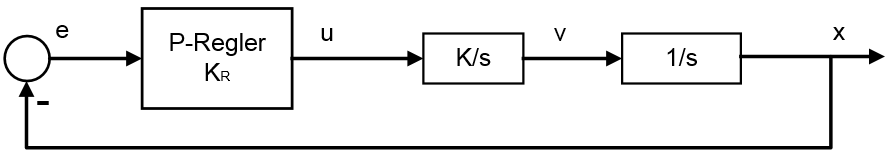
\includegraphics[width=4.6in]{imgs/NLR20.png}\\
Systempole: $F_0(s)+1=0\quad s^2+K_R\cdot K=0 \quad \Rightarrow \quad \lambda_{1,2}=\pm j\sqrt{K_R\cdot K}$\\
\uline{also:} Dauerschwingungen bei $\uline{x}_0\ne \uline{0}$, d.h. Ruhelage $\uline{x}_R= \uline{0}$ stabil, aber nicht asymptotisch stabil (vergleich Beispiel 1 von 2.2).\\
\uline{Trajektorien bei festem $K_R$:} aus Struktur $\ddot{x}=K\cdot u=-K\cdot K_R\cdot x$\\
$\Rightarrow \left.
\begin{array}{r}
\dot{x}=v\\
\dot{v}=-K_R\cdot K\cdot x
\end{array}
\right\} \Rightarrow \frac{dv}{dx}=-\frac{K\cdot K_R\cdot x}{v}$\\
Verläufe: \fbox{s. BB imgs/NLR 2-19, 2-20}
\[\frac{x^2}{\frac{c}{K\cdot K_R}}+\frac{v^2}{c}=1\]
$\Rightarrow$ \uline{Ellipsen um (0,0)}  ($a^2=\frac{c}{K\cdot K_R},\quad b^2=c$)\\
\uline{dabei:}
\[\frac{x-\text{Halbebene}}{v-\text{Halbebene}}=\frac{a}{b}=\frac{1}{\sqrt{K \cdot K_R}}\]
\[\Rightarrow\quad
\left \{%
\begin{array}{lcrcl}
     K\cdot K_R>1 & \text{d.h. } K_R>\frac{1}{K} & \Rightarrow \text{stehende Ellipsen}\\
     K\cdot K_R<1 & \text{d.h. } K_R<\frac{1}{K} & \Rightarrow "\text{liegende Ellipsen}\\
\end{array} \right.\]
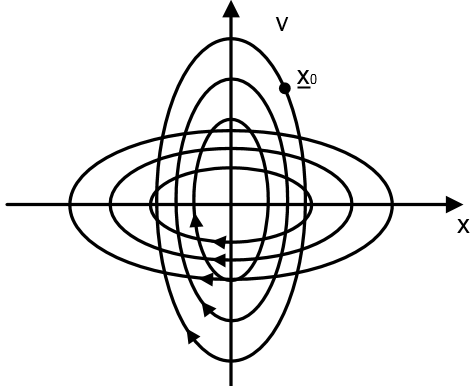
\includegraphics[width=2.2in]{imgs/NLR21.png}\\
für jedes $K_R$: Ruhelage (0,0) stabil, aber nicht asymptotisch stabil\\
\uline{jetzt:} \uline{$K_R$ umschaltbar}
\[K_R=\left \{%
\begin{array}{lcrcl}
     K_{R1}>\frac{1}{K} & \text{im 1. und 3. Quadranten}\\ 
     K_{R2}<\frac{1}{K} & \text{im 2. und 4. Quadranten}\\ 
\end{array} \right.
\]
\uline{Trajektorie: s. unten} \\
Schaltgesetz:\\
\begin{minipage}[c]{\textwidth}
\fbox{\parbox{\textwidth}{
\[K_R=\left \{%
\begin{array}{lcrcl}
     K_{R1} & x>0 \cap v>0 \quad \text{und }  x<0 \cap v<0 & \text{also:}\quad \uline{x \cdot v >0}\\ 
     K_{R2} & x>0 \cap v<0 \quad \text{und }  x<0 \cap v>0 & \text{also:}\quad \uline{x \cdot v <0}\\
\end{array} \right.\]
\[
K_R=\frac{1}{2}(K_{R1}+K_{R2})+sgn(x\cdot v)\cdot \frac{1}{2}(K_{R1}-K_{R2})
\]}}
\end{minipage}\\
\uline{Struktur:}\\
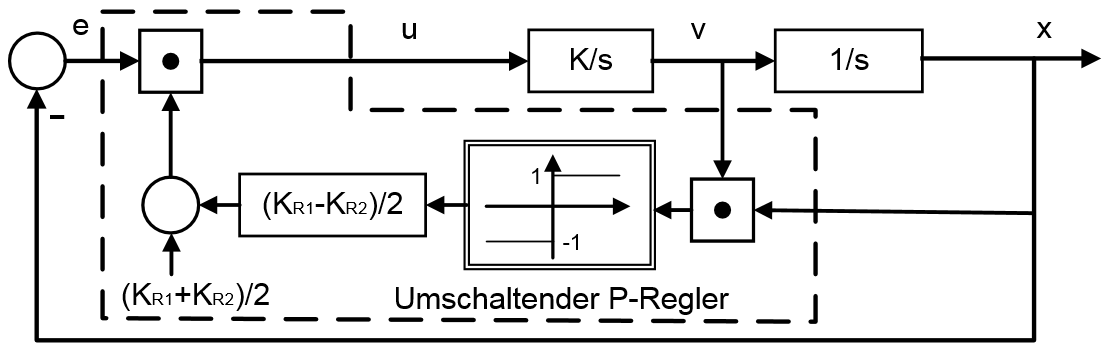
\includegraphics[width=4.8in]{imgs/NLR22.png}\\
\fbox{weitere Formen der Strukturumschaltung: z.B. Ausnutzen des Gleitvorgangs s. \uline{Föllonger}}
\section[Grenzzynklen]{Auftreten von Grenzzynklen und Zusammenhang mit der Stabilität der Ruhelage}
\uline{Grenzzyklus:} Dauerschwingungen als geschlossene Kurve C, deren Nachbartrajektorien ihr gegenüber ein Grenzverhalten zeigen.\\
\uline{3 Fälle möglich für Grenzzyklus C} \fbox{s. BB imgs/NLR 2-21, 2-22}
\begin{enumerate}
    \item \uline{asymptotisch bahnstabil:} sämtliche Trajektorien streben mit wachsender Zeit gegen C\\
    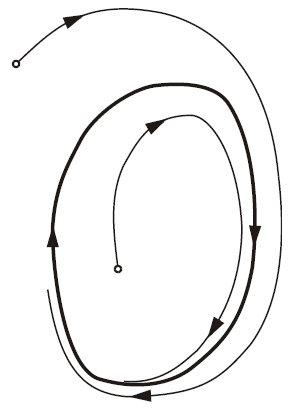
\includegraphics[width=1.4in]{imgs/NLR23.png}
    \item \uline{asymptotisch semibahnstabil:} Trajektorien streben mit wachsender Zeit nur von innen/ von außen nach C\\
    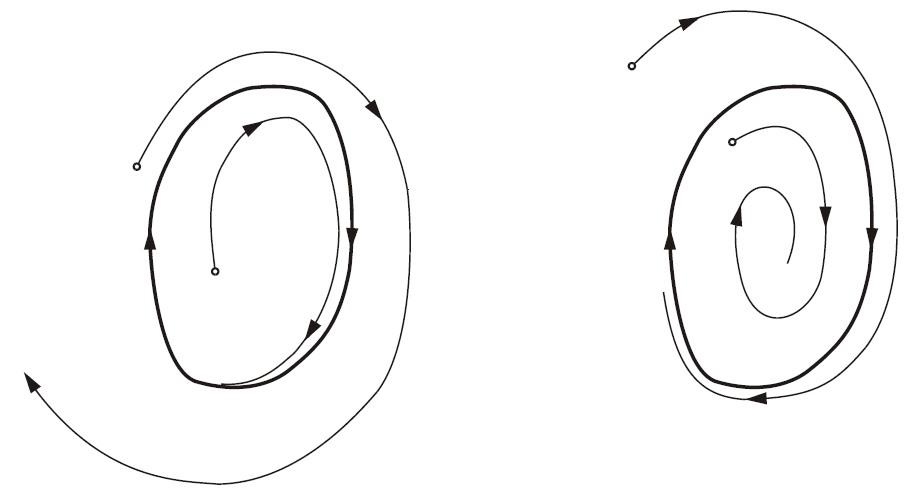
\includegraphics[width=3.2in]{imgs/NLR24.png}
    \item \uline{instabil:} Trajektorien streben mit wachsender Zeit sowohl von innen wie von außen von C weg\\
    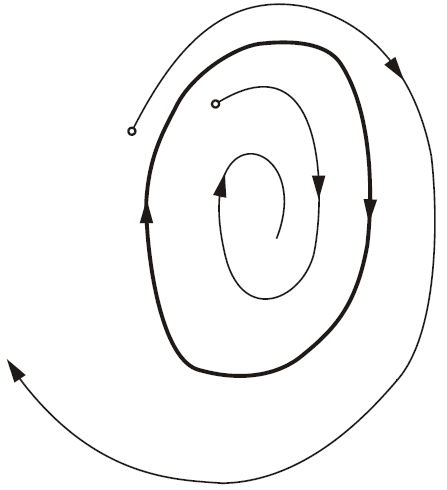
\includegraphics[width=1.6in]{imgs/NLR25.png}
\end{enumerate}
\uline{Ruhelage:} \begin{itemize}
    \item $\uline{x}_R=\uline{0}$ innerhalb von C sei einzige Ruhelage.
    \item endlich viele Grenzzyklen vorhanden C (s. oben) sei innester Grenzzyklen
\end{itemize}
1. $\uline{x}_R$ asymptotisch stabil\\
2. $\uline{x}_R$ instabil/ asymptotisch stabil\\
3. $\uline{x}_R$ instabil\\
\uline{Beispiel:}\\
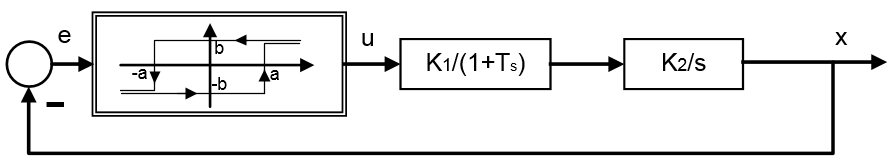
\includegraphics[width=4.6in]{imgs/NLR26.png}\\
\uline{Trajektorien(s. früher):}
\[u = \left \{%
\begin{array}{lcrcl}
     -b & ,x=-T\cdot v+K_1\cdot K_2\cdot b\cdot T\cdot ln\big|v+K_1\cdot K_2\cdot b\big|+c\\
     +b & ,x=-T\cdot v-K_1\cdot K_2\cdot b\cdot T\cdot ln\big|v-K_1\cdot K_2\cdot b\big|+c\\
\end{array} \right.
\]
\uline{Schaltlinie:}
\[u = \left \{%
\begin{array}{lcrcl}
     -b \left \{%
\begin{array}{llrcl}
     \dot{e}<0\cap e<-a & \text{d.h. } v>0\cap x>a\\
     \dot{e}>0\cap e>-a & \text{d.h. } v<0\cap x>-a\\
\end{array} \right. \\
     +b \left \{%
\begin{array}{llrcl}
     \dot{e}<0\cap e<-a & \text{d.h. } v>0\cap x<a\\
     \dot{e}>0\cap e>-a & \text{d.h. } v<0\cap x<-a\\
\end{array} \right.
\end{array} \right.
\]
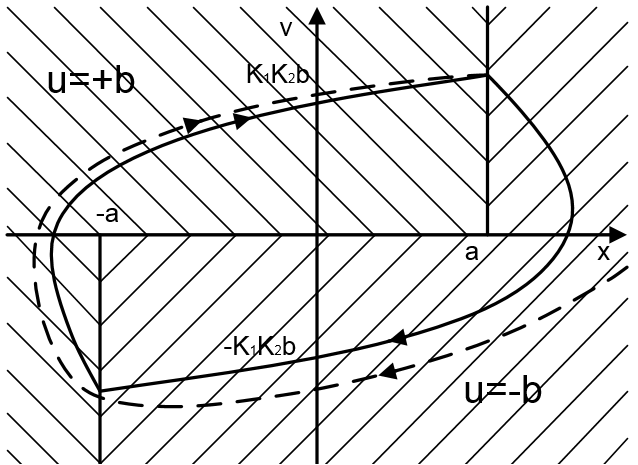
\includegraphics[width=2.4in]{imgs/NLR27.png}
\section{Totzeitsysteme in der Phasenebene}
\uline{Typische Beispiel:}\\
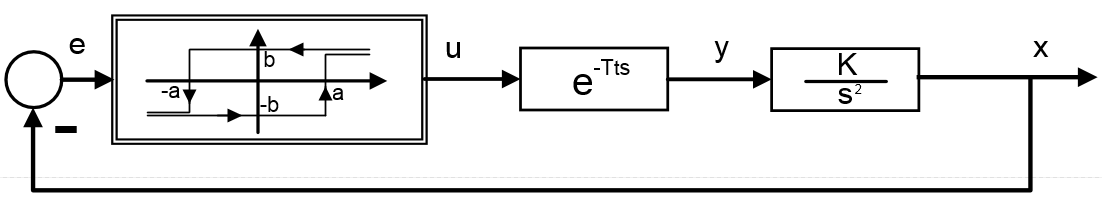
\includegraphics[width=4.6in]{imgs/NLR28.png}
\begin{enumerate}
    \item \uline{Ohne Berücksichtigung der Totzeit}
    \[X(s)=\frac{K}{s^2}\cdot Y(s) \quad \Rightarrow \quad \ddot{x}(t)=k\cdot y(t)=\pm k\cdot b\]
    \[\text{\uline{Zustandsgleichungen:}}
    \left.
    \begin{array}{r}
    \dot{x}=v\\
    \dot{v}=\pm k\cdot b
    \end{array}
    \right\} \quad \frac{dv}{dx}=\pm \frac{k\cdot b}{v}\]
    \[\text{s. früher, Parabeln: } v^2=\pm2\cdot k\cdot b\cdot x +c \quad x=0 \Rightarrow c=v_1^2\]
    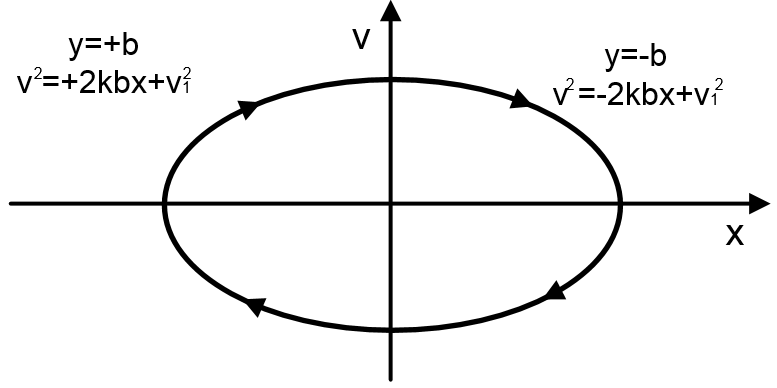
\includegraphics[width=2.6in]{imgs/NLR29.png}
    \item \uline{Berücksichtigung der Totzeit}\\
    Effekt: Umschaltung wegen Totzeit erst nach Ablauf von $T_t$ wirksam $\Rightarrow$ Trajektorie bleibt Parabel $v^2=-2\cdot k\cdot b\cdot x +v_1^2$ bis ($x_s,v_s$)\\
    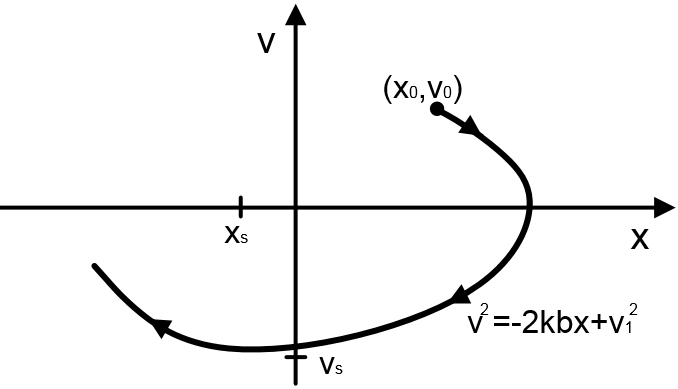
\includegraphics[width=2.4in]{imgs/NLR30.png}
    \[\text{\uline{neue Schaltlinie:}  } \frac{dv}{dt}=-k\cdot b \quad \int dt=-\int \frac{dv}{kb} \Rightarrow T_t=-\int_{v_1}^{v_s} \frac{dv}{kb}=-\frac{1}{kb}\cdot (v_s-v_1)\]
    \[ \text{bzw.: } v_1-v_s = kb\cdot T_t \quad (1)\]
    \[ \text{außerdem: } v_s^2=-2kb\cdot x_s+v_1^2 \quad (2)\]
    \[(1),(2): v_s^2=-2kb\cdot x_s+(v_s+kb\cdot T_t)^2 \Rightarrow \frac{x_s}{\frac{1}{2}kb\cdot T_t^2}-\frac{v_s}{\frac{1}{2}kb\cdot T_t}=1 \quad \text{\uline{Schaltlinie (1. Teil)}}\]
    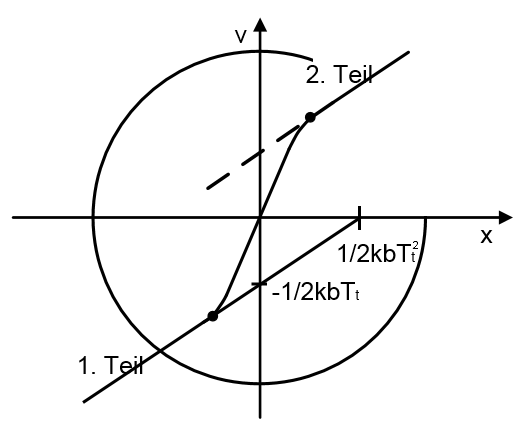
\includegraphics[width=2.8in]{imgs/NLR31.png}
\end{enumerate}
\section[Systemen höherer Ordnung]{Behandlung von Systemen höherer Ordnung in der Phasenebene}
bisherige Vorgehensweise ist ausgeschlossen, einzige Möglichkeit: \uline{Reduktion der Systemordnung} durch \uline{Approximation} (evtl. mit Totzeit)\\
Beispiel: \begin{itemize}
    \item Strecke:\\
    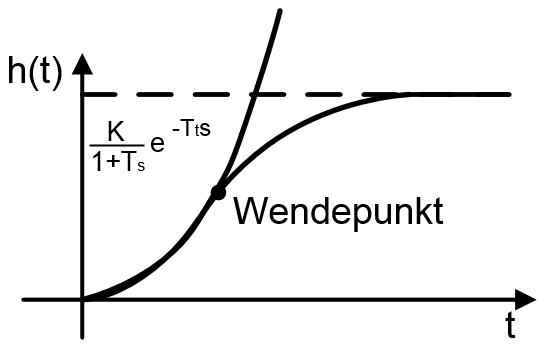
\includegraphics[width=2.8in]{imgs/NLR32.png}
    \item Stelleinrichtung: $\frac{K_s}{s}$ $\Rightarrow$ Gesamtsystem 2. Ordnung $\frac{k\cdot k_s}{s(1+T_s)}\cdot e^{-T_t\cdot s}$
\end{itemize}
durch \uline{Kaskadenregelung}\\
Beispiel: Regelung eines Gleichstromantriebs\\
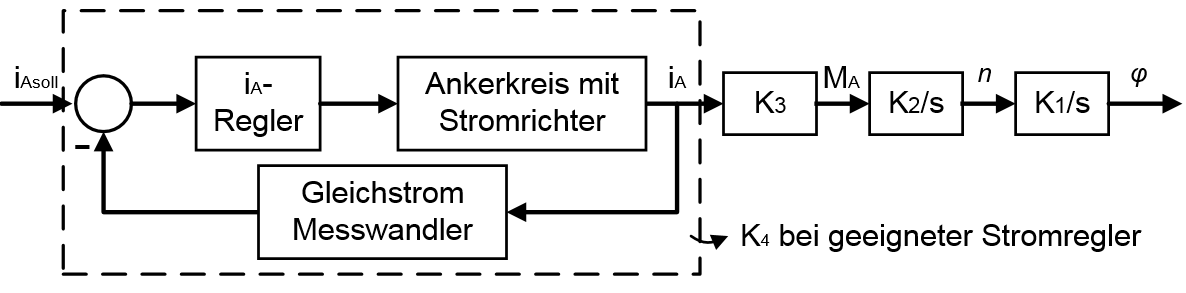
\includegraphics[width=4.6in]{imgs/NLR33.png}
%--------------------------Kapitel 3----------------------------%
\chapter[Lyapunov-Stabilität]{Analyse nichtlinearer Systeme auf Lyapunov-Stabilität}
\section[direkte Methode]{Grundgedanke der direkten Methode}
\uline{Voraussetzungen: } \begin{itemize}
    \item Dynamisches System: $\uline{\dot{x}}=\uline{f}(\uline{x})$
    \item Ruhelage: $\uline{x}_R=\uline{0}$
\end{itemize}
\uline{Prinzip: } Überprüfung der Stabilität (s. früher) von $\uline{x}_R=\uline{0}$ ohne explizite Berechnung der Trajektorien x(t)\\
\uline{Direkte Methode von Lyapunov}\\
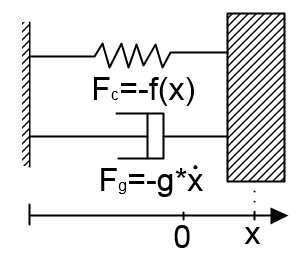
\includegraphics[width=1.4in]{imgs/NLR34.png}  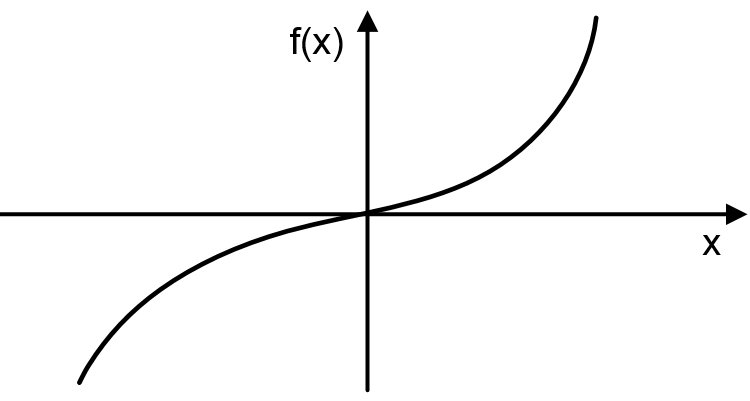
\includegraphics[width=2.4in]{imgs/NLR35.png}\\
\uline{Kräftebilanz:} $m\ddot{x}=-f(x)-g\dot{x}$\\
\uline{Zustandsgrößen:} $\left. \begin{array}{r}
    x_1=x\\
    x_2=\dot{x}\\
    \end{array}
    \right\} \Rightarrow 
    \begin{array}{l}
    \dot{x}_1=x_2\\
    \dot{x}_2=-\frac{1}{m}f(x_1)-\frac{g}{m}x_2\\
    \end{array}$\\
\uline{Ruhelagen:} $x_1=x_2=0$\\
\uline{Ansatz:} Bewegung hängt mit Energie zusammen
\[E=E_{pot}+E_{kin}=\int_x^0 -f(\xi)d\xi+\frac{1}{2}m\dot{x}^2 \Rightarrow E(x_1,x_2)=\int_0^{x_1}f(\xi)d\xi +\frac{1}{2}mx_2^2\]
E \uline{positiv definit}, d.h. E$\ge$0 (E=0, nur wenn $x_1$=0, $x_2$=0)
\[\dot{E}=f(x_1)\dot{x}_1+mx_2\dot{x}_2=f(x_1)x_2+mx_2[-\frac{1}{m}f(x_1)-\frac{g}{m}x_2]=-gx_2^2\le 0\]
\[\Rightarrow \dot{E}=0 \Rightarrow x_2=0\Rightarrow\dot{x}_2=0\Rightarrow f(x_1)=0\Rightarrow x_1=0\]
\uline{also:} \begin{itemize}
    \item Energie nimmt monoton ab
    \item Abnahme erst beendet in $\uline{x}=\uline{0}$
\end{itemize}
$\Rightarrow$ Ruhelage $\uline{x}_a=\uline{0}$ global asymptotisch stabil\\
\uline{Ansatz von Lyapunov(1898):}\\
Statt Energie Wahl einer allgemeinen Funktion $V(x)$, für die gilt:\\
$\left. \begin{array}{r}
    V(\uline{x}) \text{ positiv definit}\\
    \dot{V}(\uline{x}) \text{ negativ definit}\\
    \end{array}
    \right\} \Rightarrow \text{\uline{V(\uline{x}): Lyapunov-Funktion}}$\\
\uline{Grundgedanke der direkten Methode:}\\
\begin{minipage}[c]{\textwidth}
\fbox{\parbox{\textwidth}{
Wenn es gelingt für ein System $\uline{\dot{x}}=\uline{f}(\uline{x})$ mit $\uline{x}_R=\uline{0}$ eine derartige Lyapunov-Funktion $V(\uline{x})$ für eine Umgebung um $\uline{x}_R$ zu finden, so ist $\uline{x}_R$ global asymptotisch stabil}}
\end{minipage}
\uline{Ziel:} Ermittelung einer allgemeinen Funktion $V(\uline{x})$ (Lyapunov-Funktion) für die gilt: $V(\uline{x})$ positiv definit \& $\dot{V}(\uline{x})$ negativ definit in einer Umgebung der Ruhelage $\uline{x}_R=\uline{0}$ $\Rightarrow$ $\uline{x}_R$ asymptotisch stabil
\section{Stabilitätskriterium (nach Lyapunov)}
\uline{A) Stabilitätstheorem nach Lyapunov}(Föllinger: Stabilität im kleinen) \fbox{s. BB imgs/NLR 3-1}\\
\uline{Plausibilitätsbetrachtung für n=2}\\
$V(x_1,x_2)=c$,  $c>0$, Niveau-(Höhen-)Linien von $V$\\
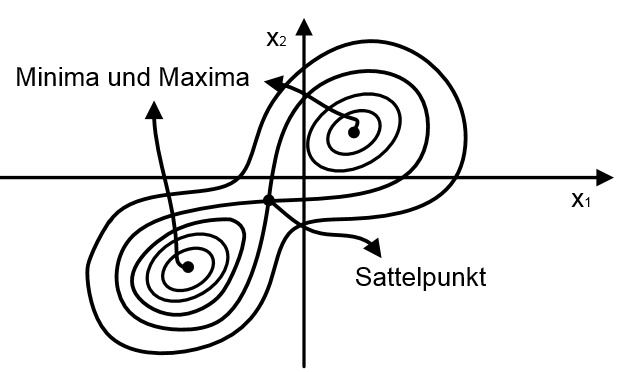
\includegraphics[width=3in]{imgs/NLR36.png}\\
Annahme: nur eine Ruhelage in $\uline{x}=\uline{0}$, c $\uparrow$ mit $|\uline{x}|$ $\uparrow$, $\dot{V}<0$, $V>0$ $\Rightarrow$ V monoton fallend $\Rightarrow$ $\uline{x}(t)\rightarrow\uline{0}$: asymptotisch stabile Ruhelage $\uline{x}_R$\\
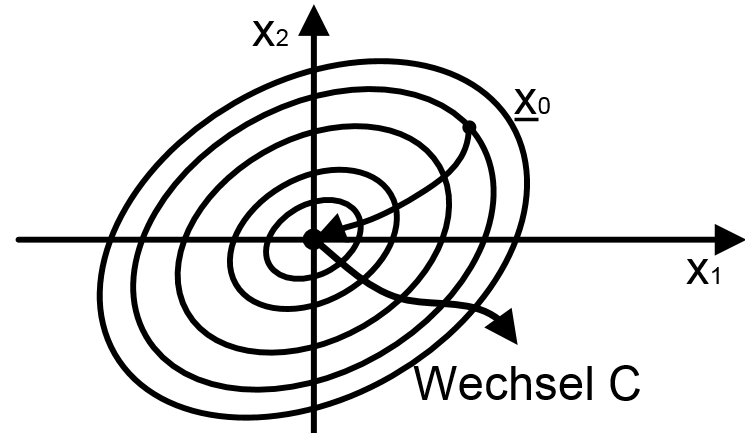
\includegraphics[width=2.4in]{imgs/NLR37.png}\\
\uline{Teilbeweis:} (für Stabilität)\\
\[\forall \varepsilon>0 \quad \exists \delta =\delta(\varepsilon)>0: \quad ||\uline{x}(0)||<\delta \Rightarrow ||\uline{x}(f)||<\varepsilon \text{ (s. früher)}\]
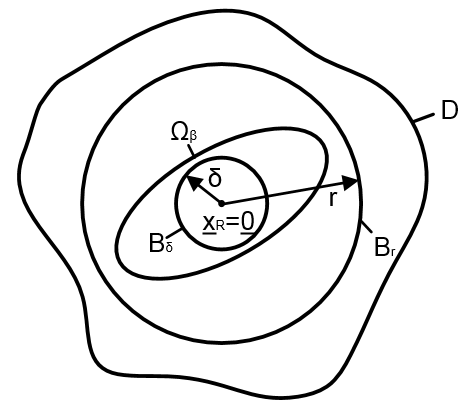
\includegraphics[width=2.3in]{imgs/NLR38.png}
\begin{enumerate}
    \item $\varepsilon>0$: $r \in (0,\varepsilon]$ mit $B_r=\{\uline{x} \in \mathbb{R}^n\big|\quad ||\uline{x}||\le r\}$
    \item $\alpha=\underset{||\uline{x}||=r}\min V(\uline{x})$ (>0 wegen $V(\uline{x})$>0 in $D-\{\uline{0}\}$)\\
    $\beta \in (0,\alpha)$ mit $\Omega_\beta =\{\uline{x}\in B_r |\quad V(\uline{x})\le \beta\}$\\
    \uline{1. Fall:} $\dot{V}(x)\le 0$ $\Rightarrow$ $V(\uline{x}(t))\le V(\uline{x}(0)) \le \beta \quad \forall t>0$
    \item $\delta_{max}=\underset{V(\uline{x})=\beta}\min||\uline{x}||$ \quad $\delta \in (0,\delta_{max})$ mit $B_{\delta}= \{ x \in \Omega_\beta \big| \quad ||\uline{x}||\le \delta \} $\\
    damit gilt: $B_\delta \subset \Omega_\beta \subset B_r$, $\uline{x}(0)\in B_\delta$ $\Rightarrow$ $\uline{x}(0)\in \Omega_\beta$ $\Rightarrow$ $\uline{x}(t)\in \Omega_\beta$ $\Rightarrow$ $\uline{x}(t)\in B_r$\\
    \uline{also:} $||\uline{x}(0)||<\delta$ $\Rightarrow$ $||\uline{x}(t)||<r\le \varepsilon$ \quad $\forall t>0$ \\
    d.h. $\uline{x}_R=\uline{0}$ stabil\\
    \uline{2. Fall:} $\dot{V}(\uline{x})<0$: $\uline{x}(t) \rightarrow \uline{0}$ d.h. $\uline{x}_R=\uline{0}$ asymptotisch stabil
\end{enumerate}
\uline{Probleme:}\begin{itemize}
    \item Lyapunov-Funktion $V(\uline{x})$ zu finden: s. später
    \item \uline{Kriterium ist nur hinreichend:} keine Aussagen, wenn Stabilität mit der gewählten Lyapunov-Funktion nicht zu zeigen ist!
    \item \uline{Einzugsbereich der Ruhelage:} Beispiel:\\
    - falls $\uline{x}_R$ stabil, aber Grenzzyklus zu klein $\Rightarrow$ unbrauchbar!\\
    - falls $\uline{x}_R$ instabil, aber stabiler kleiner Grenzzyklus $\Rightarrow$ brauchbar!\\
    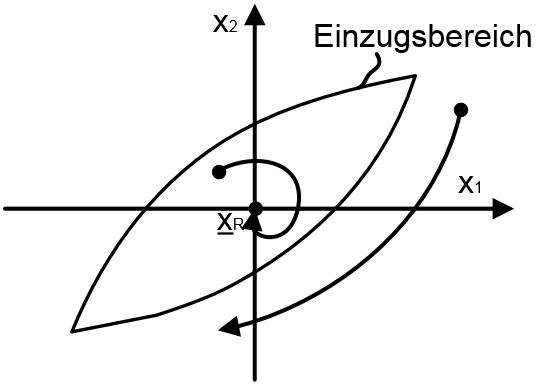
\includegraphics[width=2.1in]{imgs/NLR39.png} 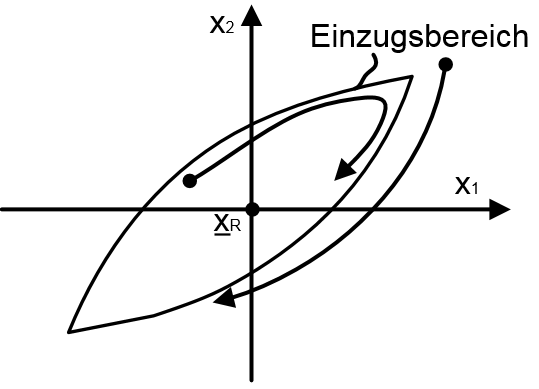
\includegraphics[width=2.1in]{imgs/NLR40.png}
\end{itemize}
\uline{also:} Abschätzung des Einzugsbereichs der Ruhelage über Vergleich mit dem Stabilitätstheorem\\
Beweis: Kriterium für asymptotisch Stabilität mit begrenztem Einzugsbereich \fbox{s. BB imgs/NLR 3-1}\\
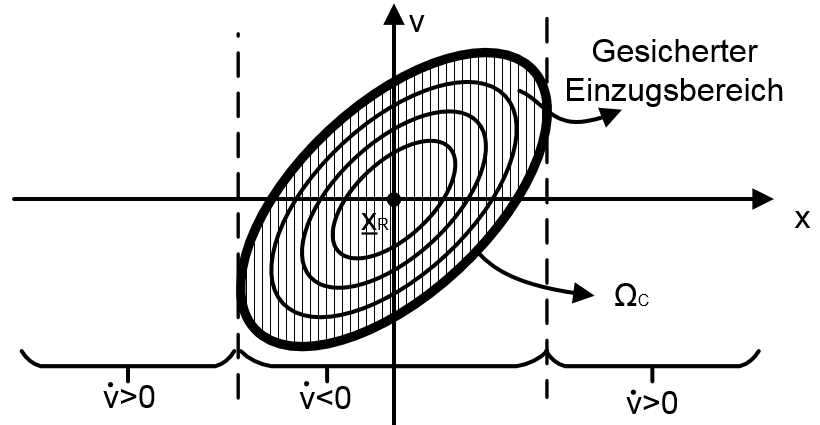
\includegraphics[width=3.2in]{imgs/NLR41.png}\\
\uline{also:} $\Omega_C$ muss nicht beschränkt sein!\\
\uline{Abhilfe:} \uline{Barbashin-Krasovskii-Theorem} \fbox{s. BB imgs/NLR 3-1}
\section[Ergänzende Kriterien]{Ergänzende Kriterien zur Stabilität und Instabilität}
\begin{enumerate}
    \item \uline{Theorem von Lasalle} \fbox{s. BB imgs/NLR 3-2}\\
    damit:  {\begin{itemize}
        \item Menge von Ruhelagen behandelbar
        \item $\dot{V}(\uline{x})\le 0$ ausreichend für asymptotisch Stabilität
        \item $V(\uline{x})$ muss nicht positiv definit sein
        \item Einzugsbereich muss nicht durch eine Lyapunov-Funktion begrenzt sein
    \end{itemize}}
    \uline{Spezialfall:} $V(x)$ positiv definit und $\uline{x}_R=\uline{0}$ behandelt \fbox{s. BB imgs/NLR 3-2 unten}
    \item \uline{Kriterium für Instabilität(Chetaevs-Theorem)} \fbox{s. BB imgs/NLR 3-3}  
\end{enumerate}
\section[Stabilitätsanalyse]{Prinzipielle Vorgehensweise zur Stabilitätsanalyse}
\begin{enumerate}
    \item \uline{Ansatz einer Lyapunov-Funktion $V(\uline{x})$ mit freien Parametern}\\
    dabei: $V(\uline{x})$ möglichest von gesamten Zustandsraum positiv definit.\\
    \uline{Beispiel:} $V=\lambda_1x_1^2+...+\lambda_nx_n^2,\quad \lambda_\upsilon(\upsilon=1,...,n)>0$
    $\Rightarrow \text{Verallgemeinerung}$
    \begin{minipage}[c]{\textwidth}
    \fbox{\parbox{\textwidth}{
    \uline{Quadrantische Formen:} $\sum_{i,k=1}^{n}P_{ik}\cdot x_i\cdot x_k=\uline{x}^T\cdot \uline{P} \cdot \uline{x}$ \\
    mit $\uline{P}=(p_{ik}) \quad \text{symmetrisch, d.h.} \quad p_{ik}=p_{ki} \quad \text{bzw.} \quad \uline{P}^T=\uline{P}$}}    \end{minipage}
    \item \uline{Bestimmung der freien Parameter von $V(\uline{x})$ Stabilitätskriterien}\\
    $\uline{x}_R$ stabil, wenn $\dot{V}(\uline{x})$ in der Umgebung der Ruhelage negativ definit.\\
    \uline{Prüfung über das Kriterium von Sylvester} \fbox{s. BB imgs/NLR 3-4}\\
    \fbox{$\dot{V}(\uline{x})$ negativ definit $\Leftrightarrow$ -$\dot{V}(\uline{x})$ positiv definit}\\
    dabei: Wahl der nach freien Parameter so, dass gesicherter Einzugsbereich möglichst groß ist!\\
    \uline{Beispiel:}\\
    $\left.
    \begin{array}{r}
    \text{System: } \dot{x}_1=-x_1+2x_1^3x_2\\
    \dot{x}_2=-x_2\\
    \end{array}
    \right\} \Rightarrow \text{Ruhelage: } \uline{x}_R=\uline{0}$\\
    1) \uline{Lyapunov-Funktion} $V(\uline{x})=\lambda_1x_1^2+\lambda_2x_2^2, \quad \lambda_1,\lambda_2>0$ (positiv definit in gesamter ($x_1,x_2$)-Ebene)\\
    Höhenlinien: $\lambda_1x_1^2+\lambda_2x_2^2=C$ bzw. $\frac{x_1^2}{c/\lambda_1}+\frac{x_2^2}{c/\lambda_2}=1$: Ellipson\\
    2) $\dot{V}(\uline{x})=2\lambda_1x_1\dot{x}_1+2\lambda_2x_2\dot{x}_2=2\lambda_1x_1(-x_1+2x_1^3x_2)+2\lambda_2x_2(-x_2)=-2\lambda_1x_1^2(1-2x_1^2x_2)-2\lambda_2x_2^2$\\
    direkt ablesbar: $\dot{V}(\uline{x})$ negativ definit, wenn $1-2x_1^2x_2>0$ bzw. $x_2<\frac{1}{2x_1^2}$\\
    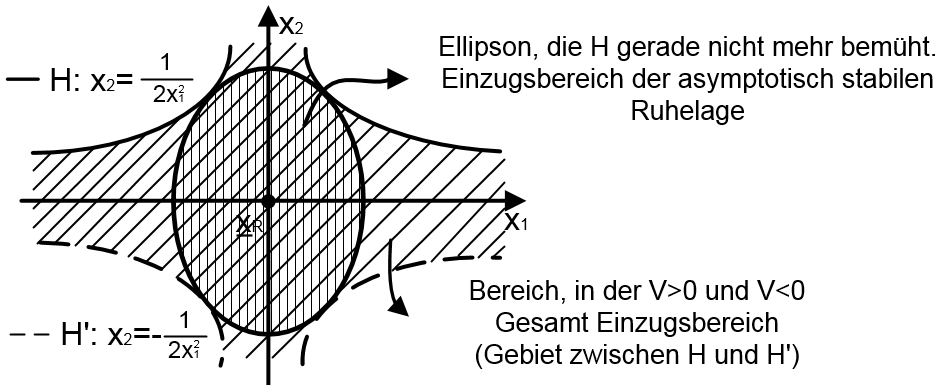
\includegraphics[width=4in]{imgs/NLR42.png}\\
    Rechnerschieb: \fbox{s. BB imgs/NLR 3-5}
\end{enumerate}
\section[Indirekte Methode]{Anwendung der Direkten Methode auf lineare Systeme und Methode der ersten Nährung (Indirekte Methode)}
Lineares System: $\dot{\uline{x}}=\uline{A}\uline{x}$\\
s. früher: $det\uline{A}\ne 0 \quad \Rightarrow$ einzige Ruhelage: $\uline{x}_R=\uline{0}$\\
$\uline{x}_R=\uline{0}$ global asymptotisch stabil, wenn alle Eigenwerte von $\uline{A}$ links der imaginären Achse liegen($\uline{A}$ ist Hurwitzmatrix).\\
\uline{Anwendung der Direkten Methode}\\
Wahl: $V(\uline{x})=\uline{x}^T\uline{P}\uline{x}$, $\uline{P}$ reellwertig, symmetrisch und positiv definit.\\
$\dot{V}(\uline{x})=\uline{x}^T\uline{P}\uline{\dot{x}}+\dot{\uline{x}}^T\uline{P}\uline{x}=\uline{x}^T\uline{P}\uline{A}\uline{x}+(\uline{A}\uline{x})^T\uline{P}\uline{x}=\uline{x}^T(\uline{P}\uline{A}+\uline{A}^T\uline{P})\uline{x}=-\uline{x}^T\uline{Q}\uline{x}$\\
nun gilt nach Lyapunov\\
Ruhelage $\uline{x}_R=\uline{0}$ asymptotisch stabil, wenn $\uline{Q}$ positiv definit, also gilt für asymptotisch Stabilität.\\
\fbox{Eigenwerte von $\uline{A}$ links der imaginären Achse $\Leftrightarrow \quad \uline{Q}=(-\uline{PA}-\uline{A^TP})$ positiv definit}\\
Wahl von \uline{Q} (reell, symmetrisch positiv definit), ungleiche Lösung der Lyapunov-Gleichung, falls Lösung $\uline{P}$ existiert (eindeutig, positiv definit) $\Leftrightarrow$ Eigenwerte von \uline{A} links der imaginären Achse (\uline{A} ist Hurwitzmatrix) $\Rightarrow$ $\uline{x}_R=\uline{0}$ asymptotisch stabil\\
\uline{Zusammenhang mit dem nichtlinearen System}\\
\uline{Nichtlineares System:} $\uline{\dot{x}}=\uline{f}(\uline{x})$, f stetig differenzierbar $\Rightarrow$ Aufspaltung in linearen und nichtlinearen Anteil möglich: $\dot{\uline{x}}=\underbrace{\uline{A}\uline{x}}_{\text{linear}}+\underbrace{\uline{g}(\uline{x})}_{\text{nichtlinear}}$\\
z.B. Taylorentwicklung von Ruhelage $\uline{x}_R$
\[\Delta\uline{\dot{x}}=\frac{\partial \uline{f}}{\partial \uline{x}}\Big|_{\uline{x}=\uline{x}_R} \Delta\uline{x}+\underbrace{\uline{\mathcal{O}}(\Delta \uline{x})}_{\text{Terme mit Ordnung} \ge 2}\]
und Übergang $\Delta\uline{x}\rightarrow\uline{x}$\\
\uline{dabei:} Abschätzung für $\uline{\mathcal{O}}(\uline{x})$ möglich (muss gelten)
\[\frac{||\uline{\mathcal{O}}(\uline{x})||}{||\uline{x}||}\rightarrow0 \text{ für } ||\uline{x}||\rightarrow 0\]
d.h. $\mathcal{J}>0$: $\mathcal{J}_r>0$, so dass $||g(\uline{x})||<\mathcal{J}||\uline{x}||$\quad  $\forall ||\uline{x}||<r$ (Lipschitz-Bedingung)\\
\uline{Kriterium für Stabilität nach der Methode der ersten Nährung(Lyapunovs indirekt Methode)} \fbox{s. BB imgs/NLR 3-6}\\
\uline{Beweis für a):}\\
\uline{Annahme:} $\uline{A}$ ist Hurwitzmatrix (alle Eigenwerte links der imaginären Achse) $\Rightarrow$ für jede gegebene positiv definite symmetreische Matreix $\uline{Q}$ gibt es eine positiv definite Lösung $\uline{P}$ der Lyapunov-Gleichung. $\uline{P}\cdot \uline{A}+\uline{A}^T\cdot \uline{P}=-\uline{Q}$\\
damit: Lyapunov-Funktion: $V(\uline{x})=\uline{x}^T\uline{P}\uline{x}$ \[\Rightarrow \quad \dot{V}(\uline{x})=\uline{x}^T\uline{P}f(\uline{x})+\uline{f}^T(\uline{x})\uline{Px}=\uline{x}^T\uline{P}[\uline{Ax}+\uline{g}(\uline{x})]+[\uline{x}^T\uline{A}^T+\underbrace{\uline{g}^T(\uline{x})]\uline{Px}}_{\uline{x}^T\uline{Pg}}\]
\[\dot{V}(\uline{x})=\uline{x}^T(\uline{PA}+\uline{A}^T\uline{P})\uline{x}+2\uline{x}^T\uline{P}\uline{g}(\uline{x})=\underbrace{-\uline{x}^T\uline{Qx}}_{\text{negativ definit}}+\underbrace{2\uline{x}^T\uline{P}\uline{g}(\uline{x})}_{\text{unbestimmt}}\]
wegen Lipschitz-Bedingung: Abschätzung möglich
\[||2\uline{x}^T\uline{Pg}(\uline{x})|| \le 2||\uline{x}^T||\cdot ||\uline{P}||\cdot ||\uline{g}(\uline{x})||<2\mathcal{J}||\uline{P}||\cdot ||\uline{x}||^2\]
\[\Rightarrow \dot{V}(\uline{x})<-\uline{x}^T\uline{Qx}+2\mathcal{J}\lambda_{max}(\uline{P})\cdot ||\uline{x}||^2 \quad \forall ||\uline{x}||<r\]
weiterhin gilt (ohne Beweis):
\[\lambda_{max}(\uline{Q})||\uline{x}||^2\ge\uline{x}^T\uline{Qx}\ge\lambda_{min}(\uline{Q})||\uline{x}||^2\]
\uline{also:} $\dot{V}(\uline{x})<\big[-\lambda_{min}(\uline{Q})+2\mathcal{J}\lambda_{max}(\uline{P})\big]||\uline{x}||^2$, $\forall ||\uline{x}||<r$\\
Wahl von $\mathcal{J}$ so, dass gilt: $\lambda_{min}(\uline{Q})-2\mathcal{J}\lambda_{max}(\uline{P})>0$ bzw. $\mathcal{J}<\frac{\lambda_{min}(\uline{Q})}{2\lambda_{max}(\uline{P})}$ \\
$\Rightarrow \quad \dot{V}(\uline{x})$ negativ definit $\Rightarrow$ \uline{nach Kriterium A:} $\uline{x}_R=\uline{0}$ asymptotisch stabil\\
\uline{Beispiel:} Rührkesselreaktor \fbox{s. BB imgs/NLR 3-7-bis 3-11}
%--------------------------Kapitel 4----------------------------%
\chapter[Synthese im Zustandsraum]{Synthese nichtlinearer Systeme im Zustandsraum}
\uline{Ziel:} Entwurf von Regelungen unter Erzielung eines gewünscheten dydamischen Verhaltens\\
\uline{Prinzip der Synthese:} \begin{enumerate}
    \item Schritt: erste nichtlineare Rückführung zur Kompensation der vorhandenen Nichtlinearitäten $\rightarrow$ lineares Verhalten des Gesamtsystems
    \item Schritt: zweite Rückführung zur Erzielung einer gewünschten Dynamik
    \item Schritt: ggf. Vorfilterentwurf zur Erzielung eines gewünschten Führungsverhaltens\\
    Verfahren: \begin{itemize}
    \item Ein-/Ausgangslinearisierung
    \item Exakte Zustandslinearisierung
    \end{itemize}
\end{enumerate}
\section[Eingrößensysteme]{Synthese nichtlinearer Eingrößensysteme}
\uline{häufig:} System nichtlinear in Zuständen, aber linear in Steurgrößen\\
$\dot{\uline{x}}=\uline{f}(\uline{x},\uline{u})\stackrel{\text{Linearität in \uline{u}}}{\Rightarrow} \dot{\uline{x}}=\uline{a}(\uline{x})+\uline{B}(\uline{x})\uline{u}$\\
$\uline{y}=\uline{c}(\uline{x}) \stackrel{\text{Eingrößensystem}}{\Rightarrow}$ \\
\begin{minipage}[c]{0.25\textwidth}
\fbox{\parbox{\textwidth}{$\dot{\uline{x}}=\uline{a}(\uline{x})+\uline{b}(\uline{x})u\\y={c}(\uline{x})$}}
\end{minipage} \quad (a, b, c: oft differenzierbar)\\
typisches Beispiel: Rührkesselreaktor \fbox{s. BB imgs/NLR 3-7}
\subsection{Der Begriff der Differenzordnung}
\uline{Mathematische Vorberechnung}\\
$y=g(x)=g(x_1,x_2,\cdots,x_n)$: Skalarfeld\\
$\dot{\uline{x}}=\uline{f}(\uline{x})$: Vektorfeld\\
$\dot{y}=\frac{dy}{dt}=\frac{\partial g}{\partial x_1}\dot{x}_1+\cdots +\frac{\partial g}{\partial x_n}\dot{x}_n=(\frac{\partial g}{\partial \uline{x}})^T\uline{f}(\uline{x})=grad^T g \uline{f}(\uline{x})$\\
\uline{Definition:} \fbox{$grad^Tg\uline{f}(\uline{x})=(\frac{\partial g}{\partial \uline{x}})^T\uline{f}(\uline{x}):=L_{\uline{f}}g(\uline{x})$} Lie-Operator (Lie-Ableitung)  (Marius Sophus Lie(1842-1899))\\
\uline{geometrische Deutung(n=2)}\\
Skalarprodukt $\Rightarrow$ Lie-Operator ist Maß dafür, inwieweit die zeitliche Ableitung der Trajektorie und der Gradient des Skalarfeldes, die gleiche Richtung zeigen.\\
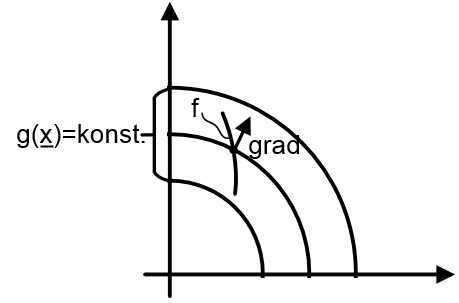
\includegraphics[width=2in]{imgs/NLR43.png}\\
\uline{Beispiel:} Lie-Operator $\dot{v}=(\frac{\partial v}{\partial \uline{x}})^T\dot{\uline{x}}=(\frac{\partial v}{\partial \uline{x}})^T\uline{f}=L_{\uline{f}}v(\uline{x})$ (s. früher)\\
\uline{Differenzordnung:} Maß für den direkten Einfluss von u auf y\\
\uline{Systemausgang:} $y=c(\uline{x})$: u triff nicht auf\\
$\dot{y}=(\frac{\partial c}{\partial \uline{x}})^T\dot{\uline{x}}=(\frac{\partial c}{\partial \uline{x}})^T[a(\uline{x})+b(\uline{x})u]\stackrel{!}{=}L_{\uline{a}}c(\uline{x})+L_{\uline{b}}c(\uline{x})u$\\
\uline{falls} $L_{\uline{b}}c(\uline{x})u=0$: \quad $\dot{y}=L_{\uline{a}}c(\uline{x})=0$\\
$\ddot{y}=\bigg(\frac{\partial\big( (\frac{\partial c}{\partial \uline{x}})^Ta(\uline{x})\big)}{\partial \uline{x}}\bigg)^T\underbrace{\dot{\uline{x}}}_{=\uline{a}(\uline{x})+\uline{b}(\uline{x})u}$ $=L_{\uline{a}}(L_{\uline{a}}c(\uline{x}))+L_{\uline{b}}(L_{\uline{a}}c(\uline{x}))u=L_{\uline{a}}^2c(\uline{x})+L_{\uline{b}}L_{\uline{a}}c(\uline{x})u$\\
\uline{falls} $L_{\uline{b}}L_{\uline{a}}c(\uline{x})=0$:\\
$\ddot{y}=L_{\uline{a}}^2 c(\uline{x})$\\
$\vdots$\\
$\stackrel{(\delta)}{y}=L_{\uline{a}}^{\delta} c(\uline{x})+\underbrace{L_{\uline{b}}L_{\uline{a}}^{\delta-1}c(\uline{x})u}_{\ne 0!}$\\
$\Rightarrow$ $\delta$=Differenzordnung des Systems (=Ordnung der wichtigsten Ableitung von $y$ auf die $u$ direkt einwirkt)\\
\uline{Formale Definition:} \fbox{s. BB imgs/NLR 4-1}\\
\uline{Beispiel:} Differenzoednung beim Rührkesselreaktor \fbox{s. BB imgs/NLR 3-7}\\
\uline{Annahme:} \\
$y=x_1=c(\uline{x})$\\
$(\frac{\partial c}{\partial \uline{x}})^T=[1,0]$ $\Rightarrow \quad L_{\uline{b}}c(\uline{x})=[1,0] \left[\begin{array}{c} 0\\ b\\ \end{array} \right]  =0$\\
$L_{\uline{a}}c(\uline{x})=[1,0]\left[\begin{array}{cc} -a_{11}x_1+\rho(x_1,x_2)\\ -a_{21}x_2+a_{22}\rho(x_1,x_2)\\ \end{array} \right]=-a_{11}x_1+\rho(x_1,x_2)$\\
$L_{\uline{b}}L_{\uline{a}}c(\uline{x})=[-a_{11}+\frac{\partial \rho}{\partial x_1} \quad \frac{\partial \rho}{\partial x_2}]\left[\begin{array}{c} 0\\ b\\ \end{array} \right] =\frac{\partial \rho(x_1,x_2)}{\partial x_2}b$\\ $=[(1-x_1)+\mu(1-x_1)^{\nu}]k_0e^{-\frac{\varepsilon}{1+x_2}}\cdot \frac{\varepsilon}{(1+x_2)^2}b$\\
(=0 nur für $x_1$=1: außerhalb des Arbeitsbereiches B)\\
\uline{also:} im Inneren von B: $\delta-1=1$, d.h. \fbox{$\delta$=2} (volle Differenzordnung!) ($\delta=n$)
\subsection{Lokale Koordinaten-Transformationen} 
\uline{Definition:} \fbox{s. BB imgs/NLR 4-2}\\
Mit Hilfe der Lie-Ableitung $L_{\uline{a}}^ic(\uline{x})$, $i=0,\cdots ,\delta-1$ lassen sich in der Umgebung $\Omega$ von $\uline{x}'$ \uline{lokale Zustandstransformationen} $\uline{z}=\uline{\Phi}(\uline{x})$ \\
durchführen mit $\Phi(\uline{x})=\left[ \begin{array}{c} \Phi_1(\uline{x})\\ \vdots\\ \Phi_n(\uline{x})\\ \end{array} \right]$, $z_i=\Phi_i(\uline{x})$\\
wobei: \begin{itemize}
    \item $i=1,\cdots,\delta$: $\Phi_i=L_{\uline{a}}^{i-1}c(\uline{x})$
    \item $i=\delta+1,\cdots,n$: $\Phi_i$ so zu wählen, dass Jacobi-Matrix $\frac{\partial \uline{\Phi}}{\partial \uline{x}}\big|_{\uline{x} \in \Omega}$ regulär\\
    $\alpha$) $\Phi_i$ aus Bedingung $L_{\uline{b}}\Phi_i=0$ (stets möglich, partielle Differentialgleichungen)\\
    $\beta$) $\Phi_i$ beliebig (unter Erfüllung der obigen Bedingung)
\end{itemize}
\begin{enumerate}
    \item $\uline{i=1,\cdots,\delta}$: $z_i=L_{\uline{a}}^{i-1}c(\uline{x})$ ($\Rightarrow z_1=c(\uline{x})=y$, allgemein $z_i=\stackrel{(i-1)}{y}$)\\
    $\Rightarrow \dot{z}_i=\underbrace{L_{\uline{a}}c(\uline{x})}_{\Phi_{i+1}}+\underbrace{L_{\uline{b}}L_{\uline{a}}^{i-1}c(\uline{x})}_{=0 \text{ für } i=1,\cdots, \delta-1}u$\\
    \fbox{$\Rightarrow \dot{z}_i=z_{i+1}$}  \quad \quad $i=1,\cdots,\delta-1$ \quad ($\Rightarrow z_{i+1}=\dot{z}_i=\stackrel{(i)}{y}, \text{ allgemein } z_i=\stackrel{(i-1)}{y}$)\\
    $i=\delta$: $\dot{z}_{\delta}=L_{\uline{a}}^{\delta}c(\uline{x})+L_{\uline{b}}L_{\uline{a}}^{\delta-1}c(\uline{x})u=\underbrace{L_{\uline{a}}^{\delta}c(\uline{\Phi}^{-1}(\uline{z}))}_{f(\uline{z})}+\underbrace{L_{\uline{b}}L_{\uline{a}}^{\delta-1}c(\uline{\Phi}^{-1}(\uline{z}))}_{g(\uline{z})}u$
    \item $\uline{i=\delta+1,\cdots,n}$: gemäß der Wahl der $\Phi_i$:\begin{itemize}
        \item $\dot{z}_i=(\frac{\partial \Phi_i}{\partial \uline{x}})^T\dot{\uline{x}}=L_{\uline{a}}\Phi_i(\uline{x})+\underbrace{L_{\uline{b}}\Phi_i(\uline{x})}_{\stackrel{!}{=}0 (\Rightarrow \Phi_i)}u\Rightarrow \dot{z}_i=L_{\uline{a}}\Phi_i(\uline{x})=\underbrace{L_{\uline{a}}\Phi_i(\uline{\Phi}^{-1}(\uline{z}))}_{:=h_i(\uline{z})}$\\
        $\Rightarrow$ 1 und 2 insgesammt: \uline{Eingangsnormalisierte Byrnes-Isidori-Normalform} \fbox{s. BB imgs/NLR 4-3}\\
        \begin{minipage}[c]{\textwidth}
        \fbox{\parbox{0.3\textwidth}{
        $\dot{z}_1=z_2$\\
        $\dot{z}_2=z_3$\\
        \vdots\\
        $\dot{z}_{\delta}=f(\uline{z})+g(\uline{z})u$\\
        $\dot{z}_{\delta+1}=h_{\delta+1}(\uline{z})$\\
        \vdots\\
        $\dot{z}_n=h_n(\uline{z})$}}
        \end{minipage}
        \item allgemeine Wahl der $\Phi_i$:\\ $\dot{z}_i=L_{\uline{a}}\Phi_i(\uline{x})+L_{\uline{b}}\Phi_i(\uline{x})u=\underbrace{L_{\uline{a}}\Phi_i(\uline{\Phi}^{-1}(\uline{z}))}_{=:h_i(\uline{z})}+\underbrace{L_{\uline{b}}\Phi_i(\uline{\Phi}^{-1}(\uline{z}))}_{:=k_i(\uline{z})}u$\\
        $\Rightarrow$ 1 und 2 insgesammt: \uline{Byrnes-Isidori-Normalform} \fbox{s. BB imgs/NLR 4-3}\\
        \begin{minipage}[c]{\textwidth}
        \fbox{\parbox{0.4\textwidth}{
        $\dot{z}_1=z_2$\\
        \vdots\\
        $\dot{z}_{\delta}=f(\uline{z})+g(\uline{z})u$\\
        $\dot{z}_{\delta+1}=h_{\delta+1}(\uline{z})+k_{\delta+1}(\uline{z})u$\\
        \vdots\\
        $\dot{z}_n=h_n(\uline{z})+k_n(\uline{z})u$}}
        \end{minipage}
        \uline{Spezialfall:} $\delta=n$:
        \begin{minipage}[c]{\textwidth}
        \fbox{\parbox{0.3\textwidth}{
        $\dot{z}_1=z_2$\\
        \vdots\\
        $\dot{z}_n=f(\uline{z})+g(\uline{z})u$}}
        \end{minipage}
        dazu: jeweils \uline{Ausgangsgleichung} \fbox{$y=z_1$} \fbox{s. BB imgs/NLR 4-3}
    \end{itemize}
\end{enumerate}
\subsection{Ein-/Ausgangslinearisierung}
\uline{Ziel:} Lineares Verhalten zwischen Ein- und Ausgangsgrößen des Sysytems mit Diffrenzordnung $\delta$ bei $\uline{x}'$ in der Umgebung $\Omega$
\begin{enumerate}
    \item \uline{Volle Diffrenzordnung $\delta=n$}\\
    $\dot{\uline{x}}=a(\uline{x})+b(\uline{x})u$\\
    $y=c(\uline{x})$\\
    $\Rightarrow$ Transformation auf Byrnes-Isidori-Normalform: $\uline{z}=\uline{\Phi}(\uline{x})$\\
    \begin{minipage}[c]{\textwidth}
        \fbox{\parbox{0.3\textwidth}{
        $\dot{z}_1=z_2$\\
        $\dot{z}_2=z_3$\\
        \vdots\\
        $\dot{z}_{n-1}=z_n$\\
        $\dot{z}_n=f(\uline{z})+g(\uline{z})u$}}
    \end{minipage}
    zusätzliche Annahme: $\uline{z}'=\uline{\Phi}(\uline{x}')=\uline{0}$ (erfüllt, wenn $\uline{x}'$ Ruhelage mit $c(\uline{x}')=0$)\\
    \uline{Rückführung:} $u=-\frac{1}{g(z)}[u_1(\uline{\uline{z}})+u_2(\uline{z})-v(\uline{z})\omega]$ (darin $g(\uline{z})\ne0$ aus Definition der Differenzordnung)\\
    mit \begin{itemize}
        \item $u_1(\uline{z})$ Kompensation der Nichtlinearitäten\\
        \fbox{$u_1(\uline{z})=f(\uline{z})$} $\Rightarrow$  $\dot{z}_n=-u_2(\uline{z})+v(\uline{z})\omega$
        \item $u_2(\uline{z})v(\uline{z})$ Vorgabe einer linearen Dynamik mit gew. Führungsverhalten\\
        \fbox{$u_2(\uline{z})=q_0z_1+\cdots+q_{n-1}z_n$} $\Rightarrow$ $\dot{z}_n=-\sum_{\nu=0}^{n-1}q_{\nu}z_{\nu+1}+v(\uline{z})\omega$\\
        ($\Rightarrow$ transformierte Gesamtsystem linear und steuerbar)
    \end{itemize}
    z.B. durch geeignete Wahl der $q_{\nu},\quad (\nu=0,\cdots,n-1)$ (z.B. durch Polvorgabe) System stabilisierbar\\
    \fbox{$\nu(\uline{z})=q_0$} (stationäre Genauigkeit)\\
    $\Rightarrow$ $\dot{z}_n=-\sum_{\nu=0}^{n-1}q_{\nu}z_{\nu+1}+q_0\omega$\\
    $\circ-\bullet \mathcal{L}$ mit $z_i=\stackrel{(i-1)}{y}$\\
    \[s^ny(s)=-\sum_{\nu=0}^{n-1}q_{\nu} s^{\nu}y(s)+q_0\omega(s) \text{ bzw. } y(s)=\frac{q_0}{s^n+q_{n-1}s^{n-1}+\cdots+q_0}\omega(s)\]
    Regelung in ursprünglichen Koordinaten:\\
    $u(\uline{z})$ $\stackrel{\uline{z}=\uline{\Phi}(\uline{x})}{\Rightarrow}$\\
    \fbox{$\Rightarrow$ $u(\uline{x})=-\frac{1}{L_{\uline{b}}L_{\uline{a}}^{n-1}c(\uline{x})}[L_{\uline{a}}^nc(\uline{x})+\sum
    _{\nu=0}^{n-1}q_{\nu}L_{\uline{a}}^{\nu}c(\uline{x})-q_0\omega]$}\\
    \uline{Nichtlineares Regelungsgesetz} sorgt für lineares, stabiles und stationär genaues Ein-/Ausgangsverhalten (und wegen $\delta=n$ auch Gesamtsystem):\\
    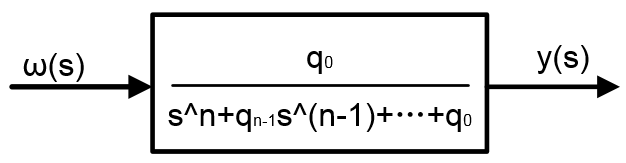
\includegraphics[width=2.2in]{imgs/NLR44.png}\\
    \uline{Ein-/Ausgangslinearisierung}\\
    \uline{aber:} häufig $\delta<n$!
    \item \uline{Diffrenzordnung $\delta<n$}\\
    wie bei (1): \\
    $\dot{\uline{x}}=a(\uline{x})+b(\uline{x})u$\\
    $y=c(\uline{x})$\\
    $\Rightarrow$ Transformation 
    $\uline{z}=\uline{\Phi}(\uline{x})$\\
    \begin{minipage}[c]{\textwidth}
        \fbox{\parbox{0.4\textwidth}{
        $\dot{z}_1=z_2$\\
        $\vdots$\\
        $\dot{z}_{\delta-1}=z_{\delta}$\\
        $\dot{z}_{\delta}=f(\uline{z})+g(\uline{z})u$\\
        $\dot{z}_{\delta+1}=h_{\delta+1}(\uline{z})+k_{\delta+1}(\uline{z})u$\\
        $\vdots$\\
        $\dot{z}_n=h_n(\uline{z})+k_n(\uline{z})u$}}
    \end{minipage}
    ($k_i(\uline{z})u$ evtl. =0 bei eingangsnormalisierte Byrnes-Isidori-Normalform)\\
    Rückführung analog zu 1.\\
    $u(\uline{z})=-\frac{1}{g(\uline{z})}[f(\uline{z})+\sum
    _{\nu=0}^{\delta-1}q_{\nu}z_{\nu+1}-q_0\omega]$\\ bzw.\\
    \fbox{$u(\uline{x})=-\frac{1}{L_{\uline{b}}L_{\uline{a}}^{\delta-1}c(\uline{x})}[L_{\uline{a}}^{\delta}c(\uline{x})+\sum
    _{\nu=0}^{\delta-1}q_{\nu}L_{\uline{a}}^{\nu}c(\uline{x})-q_0\omega]$}\\
    sorgt für partiell lineares Verhalten (in nur $\delta$ Zustandsgrößen) \uline{bezüglich des Ein-/Ausgangsverhaltens}\\
    \uline{Ein-/Ausgangslinearisierung:} \\
    \uline{Struktur:} \fbox{s. BB imgs/NLR 4-4} \\
    \uline{Beispiel:} \fbox{s. BB imgs/NLR 4-5 bis 4-9}\\
    \uline{Problem im Fall 2:} $(n-\delta)$-dimensionales Subsystem am Systemausgang nicht beobachtbar, aber durchaus von Bedeutung für die Dynamik des Gesamtsystems (evtl. instabil). Analyse dieses nichtbeobachtbaren Systems erfordlich!
\end{enumerate}
\uline{Fazit:} Analyse des nichtbeobachtbaren Systemteils ($n-\delta$ Zustandsgleichungen) erfordlich!
\subsection{Die Nulldynamik} \fbox{s. BB imgs/NLR 4-10 bis 4-11}\\
Unterscheidung der Systemanteile: $\uline{z}= \left[ \begin{array}{c} z_1\\ z_2\\ \vdots\\ z_{\delta}\\ z_{\delta+1}\\ \vdots\\ z_n\\ \end{array} \right]$ \\
darin $\uline{\xi}= \left[ \begin{array}{c} z_1\\ z_2\\ \vdots\\ z_{\delta}\\ \end{array} \right]$ und $\uline{\eta}= \left[ \begin{array}{c} z_{\delta+1}\\ \vdots\\ z_n\\ \end{array} \right]$\\
$\Rightarrow$ transformiertes System:  
    \begin{minipage}[c]{\textwidth}
    \fbox{\parbox{0.4\textwidth}{
    $\dot{z}_1=z_2$\\
    $\vdots$\\
    $\dot{z}_{\delta-1}=z_{\delta}$\\
    $\dot{z}_{\delta}=f(\uline{\xi},\uline{\eta})+g(\uline{\xi},\uline{\eta})u$\\
    $\dot{\eta}=\uline{h}(\uline{\xi},\uline{\eta})+\underbrace{\uline{k}(\uline{\xi},\uline{\eta})u}_{evtl. =0}$}}
    \end{minipage}
bei früheren Annahmen (s. 4.1.3): \begin{itemize}
    \item $\uline{x}_e'$ Ruhelage
    \item $c(\uline{x}_e')=0$
\end{itemize}   
$\Rightarrow$ $\uline{z}'=\left[ \begin{array}{c}\uline{\xi}\\ \uline{\eta}\\ \end{array}\right] '=\uline{0}$\\
$\Rightarrow$ falls $u=0$: $f(\uline{\xi}',\uline{\eta}')=\uline{0}$\\
Problem: Wahl von u so, dass für die Ausgangsgröße gilt: \fbox{$y(t)\equiv 0,\quad \forall t$}\\
$y(t)=0$ $\Rightarrow$ $z_1(t)=y(t)=0$ $\Rightarrow$ $\dot{z}_1(t)=\cdots=\dot{z}_{\delta-1}(t)=0$ $\Rightarrow$ $z_2(t)=\cdots=z_{\delta}(t)=0$\\
\uline{also:} \fbox{$\uline{\xi}(t)=\uline{0}, \quad \forall t$}\\
\uline{Bestimmung von u(t):}\begin{itemize}
    \item $\uline{k}(\uline{\xi},\uline{\eta})=\uline{0}$\\
    $\dot{z}_{\delta}=0=f(\uline{0},\uline{\eta}(t))+g(\uline{0},\uline{\eta}(t))u(t)$\\
    $\Rightarrow$ \fbox{$u(t)=-\frac{f(\uline{0},\uline{\eta}(t))}{g(\uline{0},\uline{\eta}(t))}$}\\
    Dynamik von $\uline{\eta(t)}:$ \fbox{$\uline{\dot{\eta}}(t)=\uline{h}(\uline{0},\uline{\eta}(t))$}  ($\uline{\eta}(t_0)=\eta_0$ beliebig) $\Rightarrow$ Nulldynamik\\
    \uline{also:} Nulldynamik = dynamisches Verhalten von $n-\delta$ Zustandsgrößen bei y(t)=0 $\forall t$\\
    Namensgebung: aus Vergleich mit linearen Systemen (ohne Herleitung)\\
    \uline{Lineares SISO-System mit $\delta<n$:} \\
    $n-\delta$ Zustandsgleichungen gehorchen einer linearen Dynamik $\dot{\uline{\eta}}=\uline{Q}\uline{\eta}$, wobei die Eigenwerte von \uline{Q} gerade gleich den \uline{Abkopplungsnullstellen} des SISO-System sind\\
    stets Nulldynamik überprüfen, falls $\delta<n$\\
    \uline{Beispiel:} \fbox{s. BB imgs/NLR 4-12 bis 4-14}
    \item $\uline{k}(\uline{\xi},\uline{\eta})\ne\uline{0}$\\
    wie vorher: $\uline{\xi}=\uline{0}$ $\forall t$ $\Rightarrow$ \fbox{$u(t)=-\frac{f(\uline{0},\uline{\eta}(t)}{g(\uline{0},\uline{\eta}(t)}$}\\
    \uline{Nulldynamik:} \fbox{$\dot{\uline{\eta}}(t)=\uline{h}(\uline{0},\uline{\eta}(t))-\uline{k}(\uline{0},\uline{\eta}(t))\frac{f(\uline{0},\uline{\eta}(t))}{g(\uline{0},\uline{\eta}(t))}$}\\
    \uline{Bedeutung der Nulldynamik(ohne Beweis)}\\
    Gegeben sei ein auf eingangsnormalisierte BINF(4.1.2) transformiertes System mit $\delta<n$ und der Ruhelage $\uline{z}_R=\left[ \begin{array}{c} \uline{\xi}\\ \uline{\eta}\\ \end{array} \right]_R=\uline{0}$\\
    Diesem sei mittel Ein-/Ausgangslinearisierung ein stabiles lineares Verhalten in den $\delta$ Zustandsgrößen $\uline{\xi}$ aufgeprägt werden\\
    Liegt nun für die das Verhalten der übrigen $n-\delta$ Zustandsgrößen beschreibende Nulldynamik\\
    $\dot{\uline{\eta}}=\uline{h}(\uline{0},\uline{\eta}(t))$ mit $\uline{\eta}_R=\uline{0}$ eine asymptotisch stabile Ruhelage vor, so ist die gesamte Ruhelage $\uline{r}_R$ ebenfalls asymptotisch stabil\\
    \uline{Anmerkung:}\\
        - mit obrigem Satz auch kritische Fälle für die Methode der ersten Nährung überprüfbar\\
        - Erweitung: Referenz-Ausgangsverhalten (s. Isidori)\\
    \uline{Beispiel:} \fbox{s. BB imgs/NLR 4-12 bis 4-14}
\end{itemize}
\subsection{Exakte Zustandslinearisierung}
\uline{Ziel:} primäre Stabilisierung des Systems\\
\uline{Problem:} \begin{itemize}
    \item bei $\delta<n$: Nulldynamik vorhanden, evtl. instabil!
    \item bei $\delta=n$: nur m Ausnahmefällen für Systemausgang $y=c(\uline{x})$ erfüllt 
\end{itemize}
\uline{Abhilfe:} Wahl einer fiktiven Ausgangsgröße $y^*=c^*(\uline{x})$, für die das System volle Differenzordnung $\delta=n$ besitzt\\
$\Rightarrow$ mit Ein-/Ausgangslinearisierung (bzgl. $y^*$) System stabilisierbar (gem. 4.1.3-1)
\section[Mehrgrößensysteme]{Synthese nichtlinearer Mehrgrößensysteme}
geradlinige Übertragung der Ergebnisse des Eingrößenfalls\\
wie dort: Linearität in Eingangsgrößen\\
$\uline{\dot{x}}=\uline{a}(\uline{x})+\uline{B}(\uline{x})\underbrace{\uline{u}}_{(p,1)}$, \\$\underbrace{\uline{y}}_{(q,1)}=\uline{c}(\uline{x})$\\
\uline{Annahme:} \fbox{p=q}
\subsection{Die Differenzordnung im Mehrgrößenfall}
\uline{bisher:} $L_{\uline{f}}g(\uline{x})=grad^Tg(\uline{x})\uline{f}(\uline{x})$\\
$\uline{F}=[\uline{f}_1(\uline{x}),\cdots,\uline{f}_p(\uline{x})]$\\
$\Rightarrow$ \fbox{$[L_{\uline{f}_1}g(\uline{x}),\cdots,L_{\uline{f}_p}g(\uline{x})]:=L_{\uline{F}}g(\uline{x})$}\\
Definition: Das Mehrgrößensystem\\ $\uline{\dot{x}}=\uline{a}(\uline{x})+\uline{B}(\uline{x})\uline{u}$\\
$\uline{y}=\uline{c}(\uline{x})$\\
hat die \uline{vektorielle Differenzordnung $\{\delta_1,\cdots,\delta_p\}$} an der Stelle $\uline{x}'$, wenn dort gilt:
\[L_{\uline{b}_j}L_{\uline{a}}^k c_i(\uline{x})=0 \quad (1\le i\le p, 1\le j\le p) \quad \forall k<\delta_i-1 \quad \big(\uline{B}(\uline{x})=[\uline{b}_1(\uline{x}),\cdots,\uline{b}_p(\uline{x})]\big)\]
d.h. es gilt:\\
\[\left.
\begin{array}{r}
L_{\uline{B}}c_i(\uline{x})=\uline{0}^T\\
\vdots\\
L_{\uline{B}}L_{\uline{a}}^{\delta-2}c_i(\uline{x})=\uline{0}^T\\
L_{\uline{B}}L_{\uline{a}}^{\delta-1}c_i(\uline{x})\ne\uline{0}^T\\
\end{array}
\right\} (1\le i\le p)\]
Die Zahl $\delta=\delta_1+\cdots+\delta_p$ bezeichnet man auch \uline{als Differenzordnung des Gesamtsystems:}\\
\[\left.
\begin{array}{r}
L_{\uline{B}}c_i(\uline{x})=\uline{0}^T\\
\vdots\\
L_{\uline{B}}L_{\uline{a}}^{\delta-2}c_i(\uline{x})=\uline{0}^T\\
L_{\uline{B}}L_{\uline{a}}^{\delta-1}c_i(\uline{x})\ne\uline{0}^T\\
\end{array}
\right\} (1\le i\le p)\]
$\delta=\delta_1+\cdots+\delta_p$ Differenzordnung Gesamtsystem \fbox{s. BB imgs/NLR 4-15}
\subsection{Lokale Zustandstransformation}
\fbox{s. BB imgs/NLR 4-16}\\
Gegeben sei ein nichtlineares Mehrgrößensystem:\\ $\uline{\dot{x}}=\uline{a}(\uline{x})+\uline{B}(\uline{x})\uline{u}$\\
$\uline{y}=\uline{c}(\uline{x})$\\
mit der vektoriellen Differenzordnung $\{\delta_1,\cdots,\delta_p\}$ $(\delta=\delta_1+\cdots+\delta_p)$ bei $\uline{x}=\uline{x}'$\\
Dann ist dort die Zustandstransformation $\uline{z}=\uline{\Phi}(\uline{x})=[\uline{\Phi}_1,\cdots,\uline{\Phi}_n]^T$ möglich, bei der gilt:\begin{itemize}
    \item $\Phi_1,\cdots,\Phi_{\delta}$: \\
    $\left[ \begin{array}{c} \Phi_1\\ \vdots \\ \Phi_{\delta}\\ \end{array} \right] \stackrel{!}{=}[\Phi_{11}(\uline{x}),\cdots, \Phi_{1\delta_1}(\uline{x}),\cdots,\Phi_{p1}(\uline{x}),\cdots,\Phi_{p\delta_p}(\uline{x})]^T$ mit\\
    \[\left.
    \begin{array}{r}
    \Phi_{11}(\uline{x}))=c_i(\uline{x})\\
    \Phi_{12}(\uline{x}))=L_{\uline{a}}c_i(\uline{x})\\
    \vdots\\
    \Phi_{1\delta_i}(\uline{x}))=L_{\uline{a}}^{\delta_i-1}c_i(\uline{x})\\
    \end{array}
    \right\} (1\le i\le p)\]
    \item $\Phi_{\delta+1},\cdots,\Phi_n$: beliebige Wahl so, dass Jacobi-Matrix $\frac{\partial \uline{\Phi}}{\partial \uline{x}}\big|_{x\in \Omega}$ regulär ist\\
    Unterschied zu SISO-System: Wahl aus $L_{\uline{B}}\uline{\Phi}_i=\uline{0}^T$ ($\Rightarrow$ eingangsnormalisierte BINF) nicht immer möglich!
\end{itemize}
analog zum SISO-System: neue Zustandsgrößen $\uline{z}=\left[ \begin{array}{c} \uline{\xi}\\\uline{\eta}\\ \end{array} \right]$ zu erhalten \fbox{s. BB imgs/NLR 4-17}
\begin{itemize}
    \item $\uline{\xi}=\left[ \begin{array}{c} \uline{\xi}_1\\ \vdots\\ \uline{\xi}_p\\ \end{array} \right]$ unterliegt den p Subsystemdynamiken für die $\uline{\xi}_i \quad(i=1,\cdots,p)$\\
    \begin{minipage}[c]{\textwidth}
    \fbox{\parbox{0.7\textwidth}{
    $\dot{\xi}_{i1}=\frac{d}{dt}\Phi_{i1}=\dot{\Phi}_{i1}=\Phi_{i2}=\xi_{i2}$\\
    $\vdots$\\
    $\dot{\xi}_{i\delta_{i-1}}=\xi_{i\delta_i}$\\
    $\dot{\xi}_{i\delta_i}=\underbrace{L_{\uline{a}}^{\delta_i}c_i\big(\uline{\Phi}^{-1}(\uline{\xi},\uline{\eta})\big)}_{:=f_i(\uline{\xi},\uline{\eta})}+\underbrace{L_{\uline{B}}L_{\uline{a}}^{\delta_i-1}c_i\big(\uline{\Phi}^{-1}(\uline{\xi},\uline{\eta})\big)}_{:=\uline{g}_i^T(\uline{\xi},\uline{\eta})}\uline{u}$}}
    \end{minipage}
    \item $\uline{\eta}=\left[ \begin{array}{c} \eta_1\\ \vdots\\ \eta_{n-\delta}\\ \end{array} \right]=\left[ \begin{array}{c} \uline{\Phi}_{\delta+1}\big(\uline{\Phi}^{-1}(\uline{\xi},\uline{\eta})\big)\\ \vdots\\ \uline{\Phi}_n\big(\uline{\Phi}^{-1}(\uline{\xi},\uline{\eta})\big)\\ \end{array} \right]$ unterlieget der Dynamik\\
    $\uline{\dot{\eta}}=\uline{h}(\uline{\xi},\uline{\eta})=\underbrace{\uline{k}(\uline{\xi},\uline{\eta})\uline{u}}_{\text{evtl. }=\uline{0}\text{ , aber nicht immer möglich!}}$
\end{itemize}
\uline{Ruhelage:} falls $\uline{x}'$ Systemruhelage und $c_i(\uline{x}')=\uline{0},\quad \forall i=0,\cdots,p$\\
$\Rightarrow$ $\uline{\xi}(\uline{x}')=\uline{0}$ und Wahl von $\uline{\eta}(\uline{x}')$ so möglich, dass $\uline{z}'=\left[ \begin{array}{c} \uline{\xi}\\ \uline{\eta}\\ \end{array} \right]'=\uline{0}$ ebenfalls Ruhelage \fbox{s. BB imgs/NLR 4-18}
\subsection{Reglersynthese: Ein-/Ausgangslinearisierung mit Entkoppelung}
\uline{Entkopplung:} $\forall i=1,\cdots,p$ gilt: Ausgang $y_i(t)$ nur von der Führungsgröße $\omega_i(t)$ abhängig, nicht von dem übrigen Führungsgröße\\
nun gilt (ohne Beweis): \uline{Entkopplung} (d.h. p entkoppelte Teilsysteme) genau dann erreichbar, wenn das nicht-lineares MIMO-System mit der vektoriellen Differenzordnung $\{\delta_1,\cdots,\delta_p\}$ an der Stelle $\uline{x}'$ dort eine \uline{reguläre Matrix} $\uline{D}^*(\uline{x})$ mit
\[\uline{D}^*(\uline{x})
=\left[ \begin{array}{c} L_{\uline{B}}L_{\uline{a}}^{\delta_1-1}c_1(\uline{x})\\ \vdots\\ L_{\uline{B}}L_{\uline{a}}^{\delta_p-1}c_p(\uline{x})\\ \end{array} \right]
=\left[ \begin{array}{ccc} L_{\uline{b}_1}L_{\uline{a}}^{\delta_1-1}c_1(\uline{x})&\cdots&L_{\uline{b}_p}L_{\uline{a}}^{\delta_1-1}c_1(\uline{x})\\
\vdots&\ddots&\vdots\\
L_{\uline{b}_1}L_{\uline{a}}^{\delta_p-1}c_p(\uline{x})&\cdots&L_{\uline{b}_p}L_{\uline{a}}^{\delta_p-1}c_p(\uline{x})\\
\end{array} \right]\]
d.h. det $\uline{D}^*(\uline{x})\big|_{\uline{x} \in \Omega}\ne \uline{0}$ \fbox{s. BB imgs/NLR 4-19}\\
\uline{Syntheseverfahren:} Ein-/Ausgangslinearisierung mit Entkopplung \begin{enumerate}
    \item $\uline{\delta=n}$ \\
    $\Rightarrow$ transformiertes System (vgl. 4.2.2)\\
    \begin{minipage}[c]{\textwidth}
    \fbox{\parbox{0.35\textwidth}{
    $\dot{\xi}_{i1}=\xi_{i2}$\\
    $\vdots$\\
    $\dot{\xi}_{i\delta_{i-1}}=\xi_{i\delta_i}$\\
    $\dot{\xi}_{i\delta_i}=f_i(\uline{\xi})+\uline{g}_i^T(\uline{\xi})\uline{u}$}}       ($i=1,\cdots,p$)
    \end{minipage}
    wie früher: lineare Dynamik gefordert: $\dot{\xi}_{i\delta_i}\stackrel{!}{=}-\sum_{\nu=0}^{\delta_i-1}q_{iv}\xi_{i\nu+1}+q_{i0}\omega_i$\\
    als Forderung:
    \[\underbrace{\left[ \begin{array}{c} 
    f_1(\xi)\\ \vdots\\ f_p(\xi)\\ \end{array} \right]}_{=\uline{f}(\uline{\xi})} +
    \underbrace{\left[ \begin{array}{c} 
    \uline{g}_1^T(\uline{\xi})\\ \vdots\\ \uline{g}_p^T(\uline{\xi})\\ \end{array} \right]}_{=\uline{D}^*(\uline{\xi}) (vgl. 4.2.1-2)} \uline{u}
    \stackrel{!}{=}-
    \underbrace{\left[ \begin{array}{c}      \sum_{\nu=0}^{\delta_1-1}q_{1\nu}\xi_{1\nu+1}\\ \vdots\\ \sum_{\nu=0}^{\delta_p-1}q_{p\nu}\xi_{p\nu+1}\\ \end{array} \right]}_{:=\uline{Q}\cdot \uline{\xi}}+
    \underbrace{\left[ \begin{array}{ccc} 
    q_{10}& &\uline{0}\\ &\ddots &\\ \uline{0}& &q_{p0}\\ \end{array} \right]}_{:=\uline{Q}_0}\uline{\omega}\]
    \[\Rightarrow \quad \uline{u}(\uline{\xi})=-\uline{D}^{*^{-1}}(\uline{\xi})[\underbrace{\uline{f}(\uline{\xi})}_{\text{Komp.}}+\underbrace{\uline{Q}\cdot\uline{\xi}}_{\text{lin. Dyn.}}-\underbrace{\uline{Q}_0\uline{\omega}}_{\text{entk. stat. Genauigkeit}}]  \text{ mit } \uline{\xi}=\uline{\Phi}(\uline{x})\]
    \[\uline{u}(\uline{x})=-\uline{D}^{*^{-1}}(\uline{x})
    \left[ \begin{array}{c}      L_{\uline{a}}^{\delta_1}c_1(\uline{x})+\sum_{\nu=0}^{\delta_1-1}q_{1\nu}L_{\uline{a}}^{\nu}c_i(\uline{x})\\ \vdots\\ L_{\uline{a}}^{\delta_p}c_p(\uline{x})+\sum_{\nu=0}^{\delta_p-1}q_{p\nu}L_{\uline{a}}^{\nu}c_p(\uline{x})\\ \end{array} \right]+ \uline{D}^{*^{-1}}(\uline{x}) \left[ \begin{array}{ccc} 
    q_{10}& &\uline{0}\\ &\ddots &\\ \uline{0}& &q_{p0}\\ \end{array} \right]\uline{\omega}
    \]
    \fbox{$\uline{u}(\uline{x})=-\uline{r}(\uline{x})+\uline{V}(\uline{x})\uline{\omega}$}\\
    \uline{Beispiel:} Ein-/Ausgangslinearisierung mit Entkopplung \uline{Struktur:} \fbox{s. BB imgs/NLR 4-20}
    \item \uline{$\delta<n$:} \\
    Berechnung von $\uline{u}$ wie bei 1., jedoch unbeobachtbare Dynamik $\uline{\dot{\eta}}=\uline{h}(\uline{\xi},\uline{\eta})+\uline{k}(\uline{\xi},\uline{\eta})\uline{u}$ vorhanden (evtl. instabil)\\
    für Stabilitätsuntersuchung der Ruhelage wie früher \uline{Untersuchung der Nulldynamik} ausreichend: es gilt(ohne Beweis): \fbox{s. BB imgs/NLR 4-17 bis 4-18}\\
    \begin{minipage}[c]{\textwidth}
    \fbox{\parbox{\textwidth}{
    Ist die \uline{Nulldynamik} $\uline{\dot{\eta}}=\uline{h}(\uline{0},\uline{\eta})-\uline{k}(\uline{0},\uline{\eta})\uline{D}^{*-1}(\uline{0},\uline{\eta})f(\uline{0},\uline{\eta})$ asymptotisch stabil bei der Ruhelage $\uline{\eta}_R=\uline{0}$, so ist auch die Ruhelage $\left[ \begin{array}{c}\uline{\xi_R}\\\uline{\eta_R}\\ \end{array} \right]=\uline{0}$ asymptotisch stabil}}
    \end{minipage}
\end{enumerate}
\uline{Anmerkungen:}\begin{itemize}
    \item für $\delta=n$ gehen 1. und 2. ineinander über
    \item Ergebnisse auch für \uline{p>q} übertragbar:\\
    Einteilung der $u_j \quad (j=1,\cdots,p)$ in q Gruppen, so dass Ausgang $y_i$ nur von Eingangsgrößeen aus der i-ten Gruppe beeinflusst (Entkoppelbarkeitsbedingung: Rang $\{\uline{D}^*\}=q$)
    \item weiterführende Aufgabenstellungen:\\
      -Referenz-Ausgangsverhalten erzielbar\\
      -bei Störungen Störentkoppelung möglich
\end{itemize}
\uline{Beispiel:} Regelung eines Roboterarmes  \fbox{s. BB imgs/NLR 4-21 bis 4-26}
%--------------------------Kapitel 5----------------------------%
\chapter[Harmonische Balance]{Harmonische Balance (Harmonische Linearisierung)}
Analyse eines Systems mit einer instabilen Ruhelage $\uline{x}_R$: \begin{enumerate}
    \item $\uline{x}(t)$ geht in eine neue Ruhelage über
    \item $\uline{x}(t)$ strebt gegen unendlich
    \item $\uline{x}(t)$ geht in eine Dauerschwingung(DS) über
\end{enumerate}
$\Rightarrow$ \uline{Faustregel}\\
\begin{minipage}[c]{\textwidth}
    \fbox{\parbox{\textwidth}{
    Hat ein technisches System nur eine Ruhelage und hat man alle wesentlichen Nichtlinrearitäten erfasst.\\
    Ruhelage global asymptotisch stabil, falls Dauerschwingung auftritt}}   
\end{minipage}
\uline{Harmonische Balance:} Verfahren zur Auffindung und Untersuchung von Dauerschwingungen in nichtlinearen Systemen
\section[Grundlagen]{Definition der Beschreibungsfunktion und die Gleichung der Harmonischen Balance}
\uline{hier betrachtet:} Nichtlinearer Standard-Regelkreis (\fbox{s. BB imgs/NLR 5-1})\\
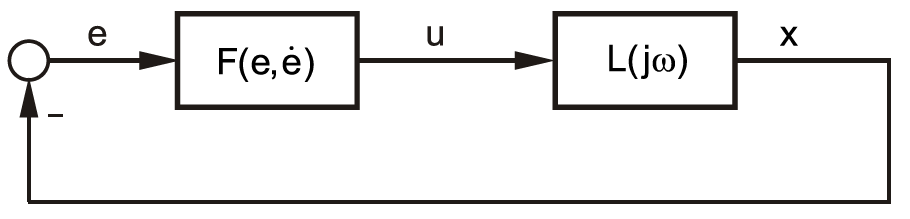
\includegraphics[width=3in]{imgs/NLR45.png}\\
\uline{Voraussetzung:} \fbox{s. BB imgs/NLR 5-1}\\
\uline{Grundannahme:} Schwingungsgleichgewicht im Regelkreis ($\Rightarrow$ Dauerschwingung mit $A_p$, $T_p=\frac{2\pi}{\omega_p}$ vorhanden)\\
\uline{dabei zusätzliche Annahme:} $\omega_p$ im Bereich der Knickfrequenzen von $L(j\omega)$\\
verboten: 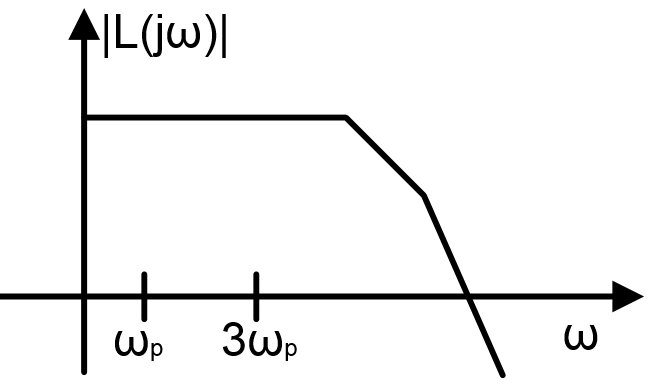
\includegraphics[width=1.6in]{imgs/NLR46.png}\\
\uline{Schwingungsgleichgewicht:} \\
\[u(t)=b_0+\sum_{\nu=1}^{\infty}\big(a_{\nu}\sin{(\nu\omega_pt)}+b_{\nu}\cos{(\nu\omega_pt)}\big)=\underbrace{b_0}_{=0}+\sum_{\nu=0}^{\infty}c_{\nu}\sin{(\nu\omega_pt+\varphi_{\nu})}\]
Durchgang durch $L(j\omega)$ $\Rightarrow$ $x(t)=\sum_{\nu=1}^{\infty}|L(j\omega_p\nu)|c_{\nu}\sin{(\nu\omega_pt+\varphi_{\nu}+\angle\!L(j\omega_p\nu))}$\\
\uline{also:} $x(t)\approx$ Grundschwingung $\Rightarrow$ auch für $u(t)$: $u(t)=c_1\sin{(\omega_pt+\varphi_1)}$\\
$u(t)=a_1\sin{(\omega_pt)}+b_1\cos{(\omega_pt)}$ $(a_1=c_1\cos{\varphi_1},\quad b_1=c_1\sin{(\varphi_1)})$\\
$\stackrel{\text{Zeigerdarstellung}}{\Rightarrow}$ $\tilde{u}=c_1e^{j(\omega t+\varphi_1)}$\\
mit $x(t)$ auch $e(t)$ eine Dauerschwingung: $e(t)=A_p\sin{(\omega_pt)}$ bzw. $\tilde{e}=A_pe^{j\omega t}$\\
\uline{Idee:} \uline{Ersatz-Frequenzgang} für die Nichtlinearität definieren (p weggelassen!)\\
\fbox{$\frac{\tilde{u}}{\tilde{e}}=\frac{c_1e^{j\varphi_1}}{A}=\frac{c_1\cos{\varphi_1}}{A}+j\frac{c_1\sin{\varphi_1}}{A}=\frac{a_1}{A}+j\frac{b_1}{A}:=N$} \uline{Beschreibungsfunktion}\\
\uline{dabei:} $a_1$, $b_1$ Fourierkoeffizienten\\
z.B. $a_1=\frac{2}{T}\int_0^T \underbrace{u(t)}_{=F(e,\dot{e})}\sin{(\omega t)}dt$ \quad\quad($F(e,\dot{e})=F(A\sin{\omega t},\omega A \cos{\omega t})$)\\
($\omega t=\nu,\quad dt=\frac{d\nu}{\omega}$) $\Rightarrow$
$=\underbrace{\frac{2}{T\omega}}_{T=\frac{2\pi}{\omega}}\int_0^{2\pi}F(A\sin{\nu},\omega A\cos{\nu})\sin{\nu}d\nu$\\
\begin{minipage}[c]{\textwidth}
    \fbox{\parbox{\textwidth}{
    $a_1=\frac{1}{\pi}\int_{0}^{2\pi}F(A\sin{\nu},\omega A\cos{\nu})\sin{\nu}d\nu =a_1(A,\omega)$\\
    analog: $b_1=\frac{1}{\pi}\int_{0}^{2\pi}F(A\sin{\nu},\omega A\cos{\nu})\cos{\nu}d\nu =b_1(A,\omega)$}}
\end{minipage}
\uline{Spezialfall:} Kennlinienglieder\\
$\Rightarrow$ $a_1(A)$, $b_1(A)$, da keine explizite Abhängigkeit von $\dot{e}$\\
$\Rightarrow$ \fbox{$N(A)=\frac{a_1(A)}{A}+j\frac{b_1(A)}{A}=R(A)+jI(A)$}\\
geschlossener Regelkreis im Schwingungsgleichgewicht:\\
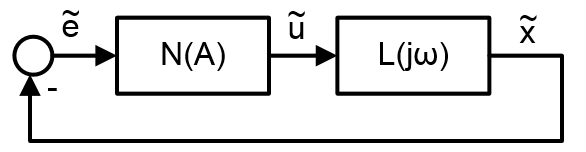
\includegraphics[width=2in]{imgs/NLR47.png}\\
$\tilde{x}=L(j\omega)N(A)\underbrace{\tilde{e}}_{=-\tilde{x}}$\\
$\Rightarrow$ \fbox{$L(j\omega)N(A)+1=0$} \uline{Gleichung der Harmonischen Balance}\\
\uline{Lösungen:}
\begin{itemize}
    \item rechnerisch (Paar reeller Gleichung für A, $\omega$)
    \item geometrisch: \uline{Zwei-Ortkurven-Verfahren}\\
    $L(j\omega)=\underbrace{-\frac{1}{N(A)}}_{:=N_I(A)}$ $\Rightarrow$ Ortskurven: $z=L(j\omega)$: lineare Ortskurve (LOK), 
    $z=N_I(A)$: nichtlineare Ortkurve (NOK)\\
    damit \uline{grafische Lösung} der Gleichung der Harmonischen Balance\\
    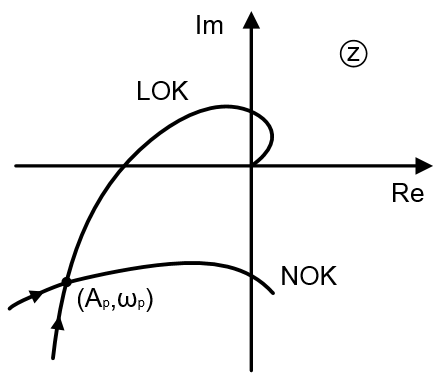
\includegraphics[width=2in]{imgs/NLR48.png}
\end{itemize}
\section[Beschreibungsfunktion \& Ortskurven]{Beschreibungsfunktion und nichtlineare Ortskurven}
\uline{Berechnung von Beschreibungsfunktion} (hier: Kennlinien)\\
aus $N(A)=R(A)+jI(A)=\frac{a_1}{A}+j\frac{b_1}{A}$\\
$\begin{array}{cc}
\text{mit}& a_1=\frac{1}{\pi}\int_{0}^{2\pi}F(A\sin{\nu},\omega A\cos{\nu})\sin{\nu}d\nu\\
& b_1=\frac{1}{\pi}\int_{0}^{2\pi}F(A\sin{\nu},\omega A\cos{\nu})\cos{\nu}d\nu\\
\end{array}$\\
\uline{Beispiel:} 
\begin{itemize}
    \item Dreipunktkennlinie\\
    \includegraphics[width=1.4in]{imgs/NLR49.png} $\Rightarrow$ $\left\{ \begin{array}{c}
    a_1=\frac{1}{\pi}\int_{0}^{2\pi}F(A\sin{\nu})\sin{\nu}d\nu\\
    b_1=\frac{1}{\pi}\int_{0}^{2\pi}F(A\sin{\nu})\cos{\nu}d\nu\\
    \end{array} \right.$\\
    Anregung mit $e=A\sin{\nu}$\\
    \includegraphics[width=2.8in]{imgs/NLR50.png}\\
    $R(A)=\frac{1}{\pi A}\int_{0}^{2\pi}\underbrace{\underbrace{u}_{ungrade}\underbrace{\sin{\nu}}_{ungerade}}_{gerade} d\nu=\frac{2}{\pi A}\int_0^{\pi} \uline{u} \sin{\nu} d\nu$\\
    $R(A)=\frac{2}{\pi A}\int_{\nu_1}^{\pi-\nu_1}b\sin{\nu} d\nu \\
    =\frac{2b}{\pi A}[-\cos{\nu}]\big|_{\nu_1}^{\pi-\nu_1}=-\frac{2b}{\pi A}[\cos{(\pi-\nu_1)}-\cos{\nu_1}]=\frac{4b}{\pi A}\cos{\nu_1}$\\
    \fbox{$R(A)=\frac{4b}{\pi A}\sqrt{1-\sin^2{\nu_1}}=\frac{4b}{\pi A}\sqrt{1-(\frac{a}{A})^2}$} \quad \fbox{$I(A)=\frac{1}{\pi A}\int_0^{2\pi}\underbrace{\underbrace{u}_{ungerade}\underbrace{\cos{\nu}}_{gerade}}_{ungerade} d\nu\stackrel{!}{=}0$}\\
    $\Rightarrow$ \fbox{$N(A)=\frac{4b}{\pi A}\sqrt{1-(\frac{a}{A})^2}$} (A$\ge$a) \uline{Beschreibungsfunktion des Dreipunktgliedes}
    \item \uline{Spezialfall:} a=0: \uline{Zweipunktglied}\\
    \fbox{$N(A)=\frac{4b}{\pi A}$} (A$\ge$0)\\
    \uline{weitere Beschreibungsfunktionen:}  \fbox{s. BB imgs/NLR 5-2 bis 5-4}\\
    \uline{Komplexer Anteil $I(A)$ von $N(A)$:} tritt auf bei Hysteresekennlinien, leicht nachzurechnen:\\
    \fbox{$I(A)=-\frac{S}{\pi A^2}$} mit S=\uline{Flächeninhalt der Hystereseschleife}
    \item \uline{Zweipunktglied mit Hysterese}\\
    \includegraphics[width=1.7in]{imgs/NLR51.png} $\Rightarrow$ $I(A)=-\frac{4ab}{\pi A^2}$\\
    Beschreibungsfunktion: \fbox{$N(A)=\frac{4b}{\pi A}\sqrt{1-(\frac{a}{A})^2}-j\frac{4ab}{\pi A^2}$}\\
    \uline{also:} Kennlinie eindeutig (S=0) $\Rightarrow$ Beschreibungsfunktion $N(A)=R(A)$ rein reell
\end{itemize}
Nichtlineare Ortkurven: \uline{NOK:} \fbox{$N_I(A)=-\frac{1}{N(A)}$}
\uline{Beispiel:}\begin{itemize}
    \item \uline{Dreipunktkennlinie}\\
    \fbox{$N_I(A)=-\frac{\pi A}{4b}\frac{1}{\sqrt{1-(\frac{a}{A})^2}}=-\frac{\pi a}{4b}\frac{(\frac{A}{a})^2}{\sqrt{(\frac{A}{a})^2-1}}$}\\
    Gestalt der Kurve (z.B. ausgewählter Punkt betrachten)\\
    \includegraphics[width=2in]{imgs/NLR52.png}
    \item \uline{Zweipunktglied}\\
    \fbox{$N_I(A)=-\frac{\pi A}{4b}$}\\
    \includegraphics[width=2in]{imgs/NLR53.png}
    \item \uline{Zeripunktglied mit Hysterese}\\
    $N_I(A)=-\frac{\pi a}{4b}\frac{1}{x\sqrt{1-x^2}-jx}$ (mit $x=\frac{a}{A}$)\\
    \fbox{$N_I(A)=-\frac{\pi a}{4b}\frac{\sqrt{1-x^2}}{x}-j\underbrace{\frac{\pi a}{4b}}_{sonst}$}\\
    \includegraphics[width=2in]{imgs/NLR54.png}
\end{itemize}
\uline{Übersicht über einige NOK:} \fbox{s. BB imgs/NLR 5-5, 5-6}
\section[Ermittlung von Dauerschwingungen]{Ermittlung von Dauerschwingungen mittels der Harmonischen Balance}
Regelkreis:\\
\includegraphics[width=3in]{imgs/NLR55.png}\\
$L(s)=\frac{K}{a_0+a_1s+\cdots+a_ns^n}$  \uline{Annahme} L2) $a_1,\cdots,a_n>0,\quad a_0\ge0$ 
\begin{enumerate}
    \item Übersicht: \uline{Zwei-Ortkurven-Verfahren}\begin{itemize}
        \item \uline{LOK-Verlauf zeichnen}\\
        \includegraphics[width=2.6in]{imgs/NLR56.png}\\
        \item \uline{NOK-Verlauf skizzieren und Schnittpunkte mit LOK bestimmen}\\
        Beispiel: Zweipunktglied\\
        \includegraphics[width=1.8in]{imgs/NLR57.png}
    \end{itemize}
    \item \uline{Rechnerische Lösung:} Gleichung der Harmonischen Balance lösen\\
    $L(j\omega_p)N(A_p)+1=0$ $\Rightarrow$ $N(A_p)=-\frac{1}{L(j\omega_p)}$ $\Rightarrow$\\
    \fbox{$\begin{array}{cc} 
    \text{Re}N(A_p)=-Re\frac{1}{L(j\omega_p)} &(1)\\
    \text{Im}N(A_p)=-Im\frac{1}{L(j\omega_p)} &(2)\\
    \end{array}$}  
\end{enumerate}
\uline{Sonderfall:} Kennlinie eindeutig\\
(2) $\Rightarrow$ \fbox{Im$\frac{1}{L(j\omega_p)}=0$}: Gleichung für $\omega_p$ allein\\
$\Rightarrow$ \fbox{$N(A_p)=-\frac{1}{L(j\omega_p)}$}: Gleichung für $A_p$ allein\\
\uline{Beispiele:} \fbox{s. BB imgs/NLR 5-7 bis 5-11}
\section[Stabilitätsverhalten]{Stabilitätsverhalten von Dauerschwingungen und Stabilität der Ruhelage}
\uline{gegeben:} Dauerschwingung mit Amplitude $A_p$ $\Rightarrow$ $A_p+\triangle A$\\
\uline{Möglichkeiten:}
\begin{enumerate}
    \item neue Dauerschwingung mit $A_p+\triangle A$
    \item{Dauerschwingung beschreibt Grenzzyklus(s. früher), der
    \begin{itemize}
        \item asymptotisch bahnstabil (Rückkehr zu Dauerschwingung mit $A_p$) $\Rightarrow$ \uline{stabile Grenzschwingung}
        \item asymptotisch semibahnstabil (Rückkehr zu Dauerschwingung nur von einer Seite) $\Rightarrow$ \uline{semistabile Grenzschwingung}
        \item instabil (Entfernung von alter Dauerschwingung) $\Rightarrow$ \uline{instabile Grenzschwingung}
    \end{itemize}}
\end{enumerate}
\uline{Beurteilung des Stabilitätsverhaltens mittels der Harmonische Balance}\\
Regelkreis im Schwingungsgleichunggewicht:\\
\includegraphics[width=2.8in]{imgs/NLR58.png}\\
Dauerschwingung: $N(A_p)\cdot L(j\omega_p)=-1$ $\Rightarrow$ $L(j\omega_p)=-\frac{1}{N(A_p)}=-\frac{1}{K_p}$\\
\includegraphics[width=1.6in]{imgs/NLR59.png}\\
neue Dauerschwingung mit $A_p+\triangle A$ ($N(A_p+\triangle A):=K$)\\
Zwei Konfigurationen möglich:\\
a) \uline{$-\frac{1}{K}>-\frac{1}{K_p}$:} LOK umschließt den Punkt $-\frac{1}{K}$ $\Rightarrow$ nach Nyquist-Kriterium liegt bei instabiler Regelkreis vor, \uline{Dauerschwingung klingt auf}\\
b) \uline{$-\frac{1}{K}<-\frac{1}{K_p}$:} $-\frac{1}{K}$ nicht von LOK umschlossen $\Rightarrow$ nach Nyquist-Kriterium liegt bei stabiler Regelkreis vor, \uline{Dauerschwingung klingt ab}\\
\uline{Zwei-Ortskurven-Darstellung:}\\
\includegraphics[width=1.8in]{imgs/NLR60.png}\\
Stabilitätskriterien für Grenzschwingungen: \fbox{s. BB imgs/NLR 5-12} \\ 
\uline{Beispiele typischer Ortskurven-Konfigurationen:}
\begin{itemize}
    \item \uline{Zweipunktglied}\\
    \includegraphics[width=2.4in]{imgs/NLR61.png}
    \item \uline{Dreipunktglied}\\
    \includegraphics[width=2in]{imgs/NLR62.png}
\end{itemize}
eigentliches Ziel: \uline{Ruhelagenanalyse}\\
n=2: Argumentation wie früher (s. Abschnitt 2.4)
\[\text{innereste Grenzschwingung} \left \{%
\begin{array}{lcrcl}
     \text{instabil} \\
     \text{stabil} \\
     \left \{%
     \begin{array}{lcrcl}
     \text{semistabil, instabil nach innen} \\
     \text{semistabil, instabil nach außen}\\
\end{array} \right.\\
\end{array} \right.\]
\[\Rightarrow \text{ Ruhelage} \left \{%
\begin{array}{lcrcl}
     \text{asymptotisch stabil} \\
     \text{instabil} \\
     \left \{%
     \begin{array}{lcrcl}
     \text{asymptotisch stabil} \\
     \text{instabil} \\
     \end{array} \right.
\end{array} \right.
\]
\uline{Beseitigung von Dauerschwingungen}\\
\uline{Beispiel:} Dreipunktglied im Regelkreis\\
\includegraphics[width=2in]{imgs/NLR63.png}\\
1) \uline{Veränderung der LOK}
\begin{itemize}
    \item Verkleinung der Kreisverstärkung(aber: Regelkreis langsamer!)
    \item Einsatz vom PD-Regler $\Rightarrow$ Phasendrehung
\end{itemize}
2) \uline{Veränderung der NOK}\\
Modifikation der Nichtlinearität\\\\
\uline{Abschluss-Anmerkungen}\\
Harmonische Balance auch anwendbar auf \uline{Regelkreis mit mehreren Kennlinien}
\begin{itemize}
    \item \uline{in Reihe} Schwingungsgleichgewicht\\
    \includegraphics[width=4in]{imgs/NLR64.png}\\
    $N_1(A)N_2(B)L_1(j\omega)L_2(j\omega)+1=0$  (2 Gleichungen)\\
    außerdem: $B=|L_1||N_1|A$ oder $A=|L_2||N_2|B$ (jeweils 1 Gleichung)\\
    $\Rightarrow$ Amplituden A,B und $\omega$ asymptotisch bestimmbar
    \item \uline{in beliebige Anordnung} mit Beschreibungsfunktionen wie mit linearer Blöcken rechenbar(aber Abkürzung von $\omega$ möglich!)\\
    \uline{Beispiel:}\\
    \includegraphics[width=4in]{imgs/NLR65.png}
\end{itemize}
\uline{aber:} stets auf Voraussetzungen der Harmonischen Balance achten! $\Rightarrow$ mehr Informationen: s. Föllinger
%--------------------------Kapitel 6----------------------------%
\chapter{Das Popov-Kriterium}
= Hinreichendes Kriterium zum Nachweis der \uline{absoluten Stabilität} nichtlinearer Regelkreise(v. M. Popov, 1959)
\section[Grundlagen]{Absolute Stabilität und Voraussetzung des Popov-Kriterium}
\uline{bisher:} Betrachtung genau definierter Nichtlinearitäten (meist Kennlinien)\\
\uline{jetzt:} lediglich Arbeitsbereich der Nichtlinearität muss bekannt sein ($\Rightarrow$ nicht exakt bekannt Kennlinien, Kennlinien-Familien behandelbar)\\
$\Rightarrow$ \uline{Absolute Stabilität} \fbox{s. BB imgs/NLR 6-1} \\ 
\uline{Voraussetzung für $L(s)$} \fbox{s. BB imgs/NLR 6-2} \\
L1) $L(s)=\frac{1}{s^p}\cdot \frac{1+b_1s+\cdots}{1+a_1s+\cdots}$, ZG<NG\\
(Kreisverstärkung V muss in $F(e)$ aufgenommen werden)\\
L2) Pole links (Hauptfall) oder allenfalls Pole \uline{auf (singulärer Fall)} der j-Achse.\\
\uline{Problem bei singulären Fall:}\\ 
durch Sektor [0, K] auch $F(e)$=0 zugelassen $\Rightarrow$ Regelkreis offen: d.h. wegen der Pole auf der j-Achse von $L(s)$, Regelkreis nicht stabil, daher auch nicht absolut stabil!\\
\uline{Abhilfe:} Übergang zum Sektor [$\varepsilon$, K] ($\varepsilon$ positiv, beliebig klein)\\
\includegraphics[width=2.2in]{imgs/NLR66.png}\\
(aber: Kennlinien mit \begin{itemize}
    \item Steigung 0 in e=0 (z.B. $u=e^3$)
    \item Steigung schwächer als Gerade in $e=+\infty$ (z.B. $u=\sqrt{e}$)
\end{itemize}
ausgeschlossen!)\\
falls Regelkreis mit $u=\varepsilon\cdot e$ global asymptotisch stabil für beliebig klein positiv $\varepsilon$: \uline{Regelkreis granzstabil}\\
\uline{also:} L3) Im singuläeren Fall sei der Regelkreis grenzstabil!
\section[Popov-Kriterium]{Formulierung und Anwendung des Popov-Kriterium}
\uline{Popov-Kriterium:} \fbox{s. BB imgs/NLR 6-2} \\
\uline{Geometrische Deutung:} (rechnerische Auswertung kompliziert!)\\
Popov-Ungleichung $\stackrel{L(j\omega)=R(\omega)+jI(\omega)}{\Rightarrow} $\\
Re$[(1+qj\omega)(R(\omega)+jI(\omega))]>-\frac{1}{K}$\\
$\Rightarrow \underbrace{ R(\omega) }_{=R_p(\omega)}-q \underbrace{\omega I(\omega)}_{=I_p(\omega)}+\frac{1}{K}>0 \quad \forall \omega \ge 0$\\
\uline{Definition:} \uline{Popov-Ortskurve} \fbox{$z=L_p(j\omega)=R_p(\omega)+jI_p(\omega)$}\\
\uline{Beispiel für Popov-Ortskurven:} \fbox{s. BB imgs/NLR 6-3} \\
Popov-Kriterium ($R_p(\omega)=:u$ $I_p(\omega)=:v$)
\[u-q\cdot v+\frac{1}{K}>0\]
\uline{Definition:} \fbox{$v=\frac{1}{q}(u+\frac{1}{K})$} \quad \uline{Popov-Gerade:} $g_p$\\
\includegraphics[width=2in]{imgs/NLR67.png}\\
also:\\
\begin{minipage}[c]{\textwidth}
\fbox{\parbox{\textwidth}{Regelkreis absolut stabil in [0, K] bzw. [$\varepsilon$, K], wenn $L_p(j\omega)$ rechts von der Popov-Gerade $g_p$ liegt}}
\end{minipage}\\
\uline{geometrisches Stabilitätskriterium}\\
\uline{Vorgehen:}\\
1. Zeichnen der Popov-Ortskurve (POK)\\
2. Einzeichnen der Popov-Gerade $g_p$\\
(dabei von links Tangente anlegen ($g_{pkrit}$) $\Rightarrow$ größstmögliches $K_p$ bestimmen)\\
\includegraphics[width=2in]{imgs/NLR68.png}\\
Grenzsektor [0, $K_p$] \uline{Popov-Sektor}\\
da $g_{pkrit}$ gemeinsam $sp_e$ mit $z=L_p(j\omega)$ aufweist\\
$\Rightarrow$ \uline{Regelkreis absolut stabil in [0, $K_p-\delta$] ($\delta$ positiv, beliebig klein)}\\
\includegraphics[width=2in]{imgs/NLR69.png}
\section[Erweiterung und Grenzen]{Erweiterung und Grenzen des Verfahrens}
A) \uline{Erweiterungen}\\
\begin{enumerate}
    \item \uline{Verallgemeinerung des Sektors}\\
    \includegraphics[width=2.2in]{imgs/NLR70.png}
    \[\Downarrow \text{\uline{Sektortransformation}}\]
    \[u^*=u-K_1e\quad \Rightarrow L^*(s)=\frac{L(s)}{1+K_1L(s)}\]
    \[F^*(e)=F(e)-K_1e\]
    \[\text{auf transformierten Regelkreis normales Verfahren anwenden (Voraussetzungen beachten!)}\]
    \includegraphics[width=2.2in]{imgs/NLR71.png}
    \item \uline{$K=+\infty$} (gesucht 1. und 3. Quadrant)\\
    $\Rightarrow$ Popov-Kriterium: $\forall \omega \ge 0$, $\exists q \in \mathbb{R}:$ \fbox{$Re[(1+qj\omega)\cdot L(j\omega)] \ge 0$} \\
    (> für Hauptfall; = für singurären Fall (nur ein Pol in s=0 zulässig))
    \item \uline{$L(s)=R(s)\cdot e^{-T_ts}$}\\
    Regelkreis absolut stabil, wenn der \uline{Hauptfall} vorliegt und ein Popov-Kriterium \fbox{$q \in \mathbb{R} >0$} existiert.
\end{enumerate}
B) \uline{Grenzen}\\
\begin{enumerate}
    \item Popov-Kriterium nur hinreichend \fbox{s. BB imgs/NLR 6-4 bis 6-10} 
    \item Nur Aussage über global asymptotisch Stabilität
\end{enumerate}
\end{document}